\part{Theoretical Framework}
\label{Part1}
The \autoref{Part1} of this thesis gives a brief introduction of the theoretical framework behind the physics programs at the \ac{LHC}, including both the \ac{SM} of particle physics and extensions of the \ac{SM} that partly motivate the physics searches discussed in \autoref{Part3} and \autoref{Part4}. Materials presented in this part of the thesis are borrowed liberally from various milestone papers and popular graduate physics textbooks, and thus shall not be considered original work of my own. The \autoref{Part1} is organized as follows. \autoref{sec:Field} introduces the field content of the standard model, including all known fermions and bosons. \autoref{sec:SM} discusses the theory of \ac{EW} interaction developed initially by Glashow, Weinberg, and Salam. The theory of strong interaction and its application to hadron colliders are discussed in \autoref{sec:QCD}. \autoref{sec:BSM} introduces several popular \ac{UV}-complete models that aims to accommodate a few fissures exposed in the \ac{SM}. Finally, a model independent framework called \ac{EFT} is discussed in \autoref{sec:EFT}.
\chapter{Field Content of the Standard Model}
\label{chap:Field}

The \ac{SM} of particle physics is a quantum field theory that combines the concept of classic field theory with quantum mechanics and Einstein's special relativity. Different elementary particles can be described as the excited states or quanta of distinct quantum fields, characterized by masses and various quantum numbers. A summary of the known elementary particles and their properties is given in Figure~\ref{fig:Field}.

\begin{figure}[tbh!]
 \begin{center}
 \begin{tabular}{c}
 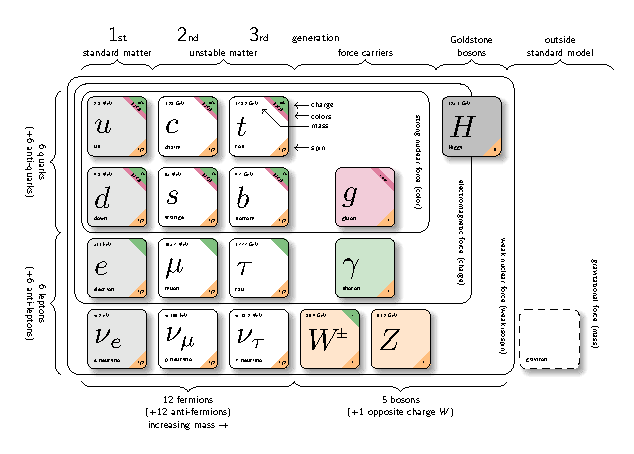
\includegraphics[width=\textwidth]{figures/Part1/Field/SM}
 \end{tabular}
 \caption{The field content of the \ac{SM}, including all known elementary particles. The three generations of fermions are shown in the first three columns. The gauge bosons that mediate the fundamental interactions are shown in the fourth and fifth columns. The sixth column shows the recently discovered Higgs boson. The hypothetical graviton that mediates gravitational force is also shown, which is outside of the realm of the \ac{SM}.~\cite{tikz:SM}}
 \label{fig:Field}
 \end{center}
\end{figure}

The effects described by special relativity apply to all elementary particles. This requires the theory to be invariant under Lorentz transformations, which contain rotations and Lorentz boosts of the coordinate systems. The behaviors of elementary particles under such transformations are characterized by their spin quantum numbers. This divides elementary particles into two groups. Those with half-integer spins are known as ``fermions''. They are fundamental building blocks of matter that exist in the universe. Particles with integer spins are known as ``bosons''. They are either mediators of the fundamental forces or are required in the mechanism that generates mass for all elementary particles. Properties of elementary fermions and bosons are discussed further in \autoref{sec:Fermion} and \autoref{sec:Boson}, respectively. 

\section{Fermions}
\label{sec:Fermion}

Named after Italian physicist Enrico Fermi, fermions follow Fermi-Dirac statistics and obey the Pauli exclusion principle, which prohibits two or more fermions with the same quantum number from simultaneously occupying the same quantum state. The matter that exists in the universe is made up of spin-$\frac{1}{2}$ fermions that can be broken into two groups, quarks and leptons. They are represented by ``spinors'' under Lorentz transformations. For example, the free Lagrangian that encodes full information of a spinor field can be expressed as,

\begin{equation}
\label{eq:lefthand}
\mathcal{L}=i\psi_{R}^{\dagger}\sigma^{\mu}\partial_{\mu}\psi_{R}
\end{equation}
or
\begin{equation}
\label{eq:righthand}
\mathcal{L}=i\psi_{L}^{\dagger}\bar{\sigma}^{\mu}\partial_{\mu}\psi_{L},
\end{equation}

where $\sigma^{\mu}$ is the 2$\times$2 Pauli matrix. The spinors in Equation~\ref{eq:lefthand}-\ref{eq:righthand} are known as Weyl spinors, which correspond to two-dimensional irreducible representations of the Lorentz group. Weyl spinors can be classified into left-handed spinors $\psi_{L}$ or right-handed spinors $\psi_{R}$ depending on the orientation of their spin relative to their momentum. More formally, $\psi_{R}$ and $\psi_{L}$ correspond to the ($\frac{1}{2}$,0) and (0,$\frac{1}{2}$) representation of the Lorentz group~\cite{zee:group}.

In addition to Lorentz invariance, the free Lagrangians should also be invariant under parity transformation. For Weyl spinors, however, this symmetry is violated as right-handed spinors transform into left-hand spinors under parity, and vice versa. To describe elementary fermions, the two irreducible representations must be stacked together, forming a four-dimensional reducible representation ($\frac{1}{2}$,0) $\bigoplus$ (0,$\frac{1}{2}$),

\begin{equation}
\label{eq:leftandright}
\mathcal{L}=i\psi_{R}^{\dagger}\sigma^{\mu}\partial_{\mu}\psi_{R}+i\psi_{L}^{\dagger}\bar{\sigma}^{\mu}\partial_{\mu}\psi_{L}.
\end{equation}

It is also possible to introduce additional Lorentz- and parity-invariant terms $m(\psi_{R}^{\dagger}\psi_{L}+\psi_{L}^{\dagger}\psi_{R})$ to Equation~\ref{eq:leftandright},

\begin{equation}
\label{eq:DiracLag}
\mathcal{L}_{Dirac}=i\psi_{R}^{\dagger}\sigma^{\mu}\partial_{\mu}\psi_{R}+i\psi_{L}^{\dagger}\bar{\sigma}^{\mu}\partial_{\mu}\psi_{L}+m(\psi_{R}^{\dagger}\psi_{L}+\psi_{L}^{\dagger}\psi_{R}),
\end{equation}

where $m$ corresponds to the physical mass of the fermions. Equation~\ref{eq:DiracLag} is known as the Dirac Lagrangian. Using the Euler-Lagrange equation that is based on the principle of least action,

\begin{equation}
\frac{\partial\mathcal{L}}{\partial\psi}-\partial_{\mu}\frac{\partial\mathcal{L}}{\partial(\partial_{\mu}\psi)}=0,
\end{equation}

the equation of motion for the Dirac Lagrangian can be written as,

\begin{equation}
\label{eq:Dirac1}
i\sigma^{\mu}\partial_{\mu}\psi_{R}=m\psi_{L}
\end{equation}
\begin{equation}
\label{eq:Dirac2}
i\bar{\sigma}^{\mu}\partial_{\mu}\psi_{L}=m\psi_{R}
\end{equation}

Defining the four-dimensional Dirac spinor as $\psi=\begin{psmallmatrix}\psi_{R}\\\psi_{L}\end{psmallmatrix}$ and the 4$\times$4 Dirac matrix as $\gamma^{\mu}=\begin{psmallmatrix}0&\bar{\sigma}^{\mu}\\\sigma^{\mu}&0\end{psmallmatrix}$, Equation~\ref{eq:Dirac1}-\ref{eq:Dirac2} can be rewritten as,

\begin{equation}
\label{eq:Dirac}
i\gamma^{\mu}\partial_{\mu}\psi-m\psi=0,
\end{equation}

which is the celebrated Dirac equation first derived by British physicist Paul Dirac~\cite{Dirac:1928hu}. Ironically, Dirac arrived at this equation with the simple goal of finding a relativistic equation with only one power of spacetime derivative and was puzzled by the negative-energy solutions to his equation. It was later understood these negative-energy solutions correspond to antiparticles that have the same mass but opposite signs of all quantum numbers. The existence of such particles was first confirmed by American physicist C. D. Anderson in 1932~\cite{PhysRev.43.491}, who used a cloud chamber to produce to first photographic evidence of positron, which is shown in Figure~\ref{fig:Positron}.

\begin{figure}[tbh!]
 \begin{center}
 \begin{tabular}{c}
 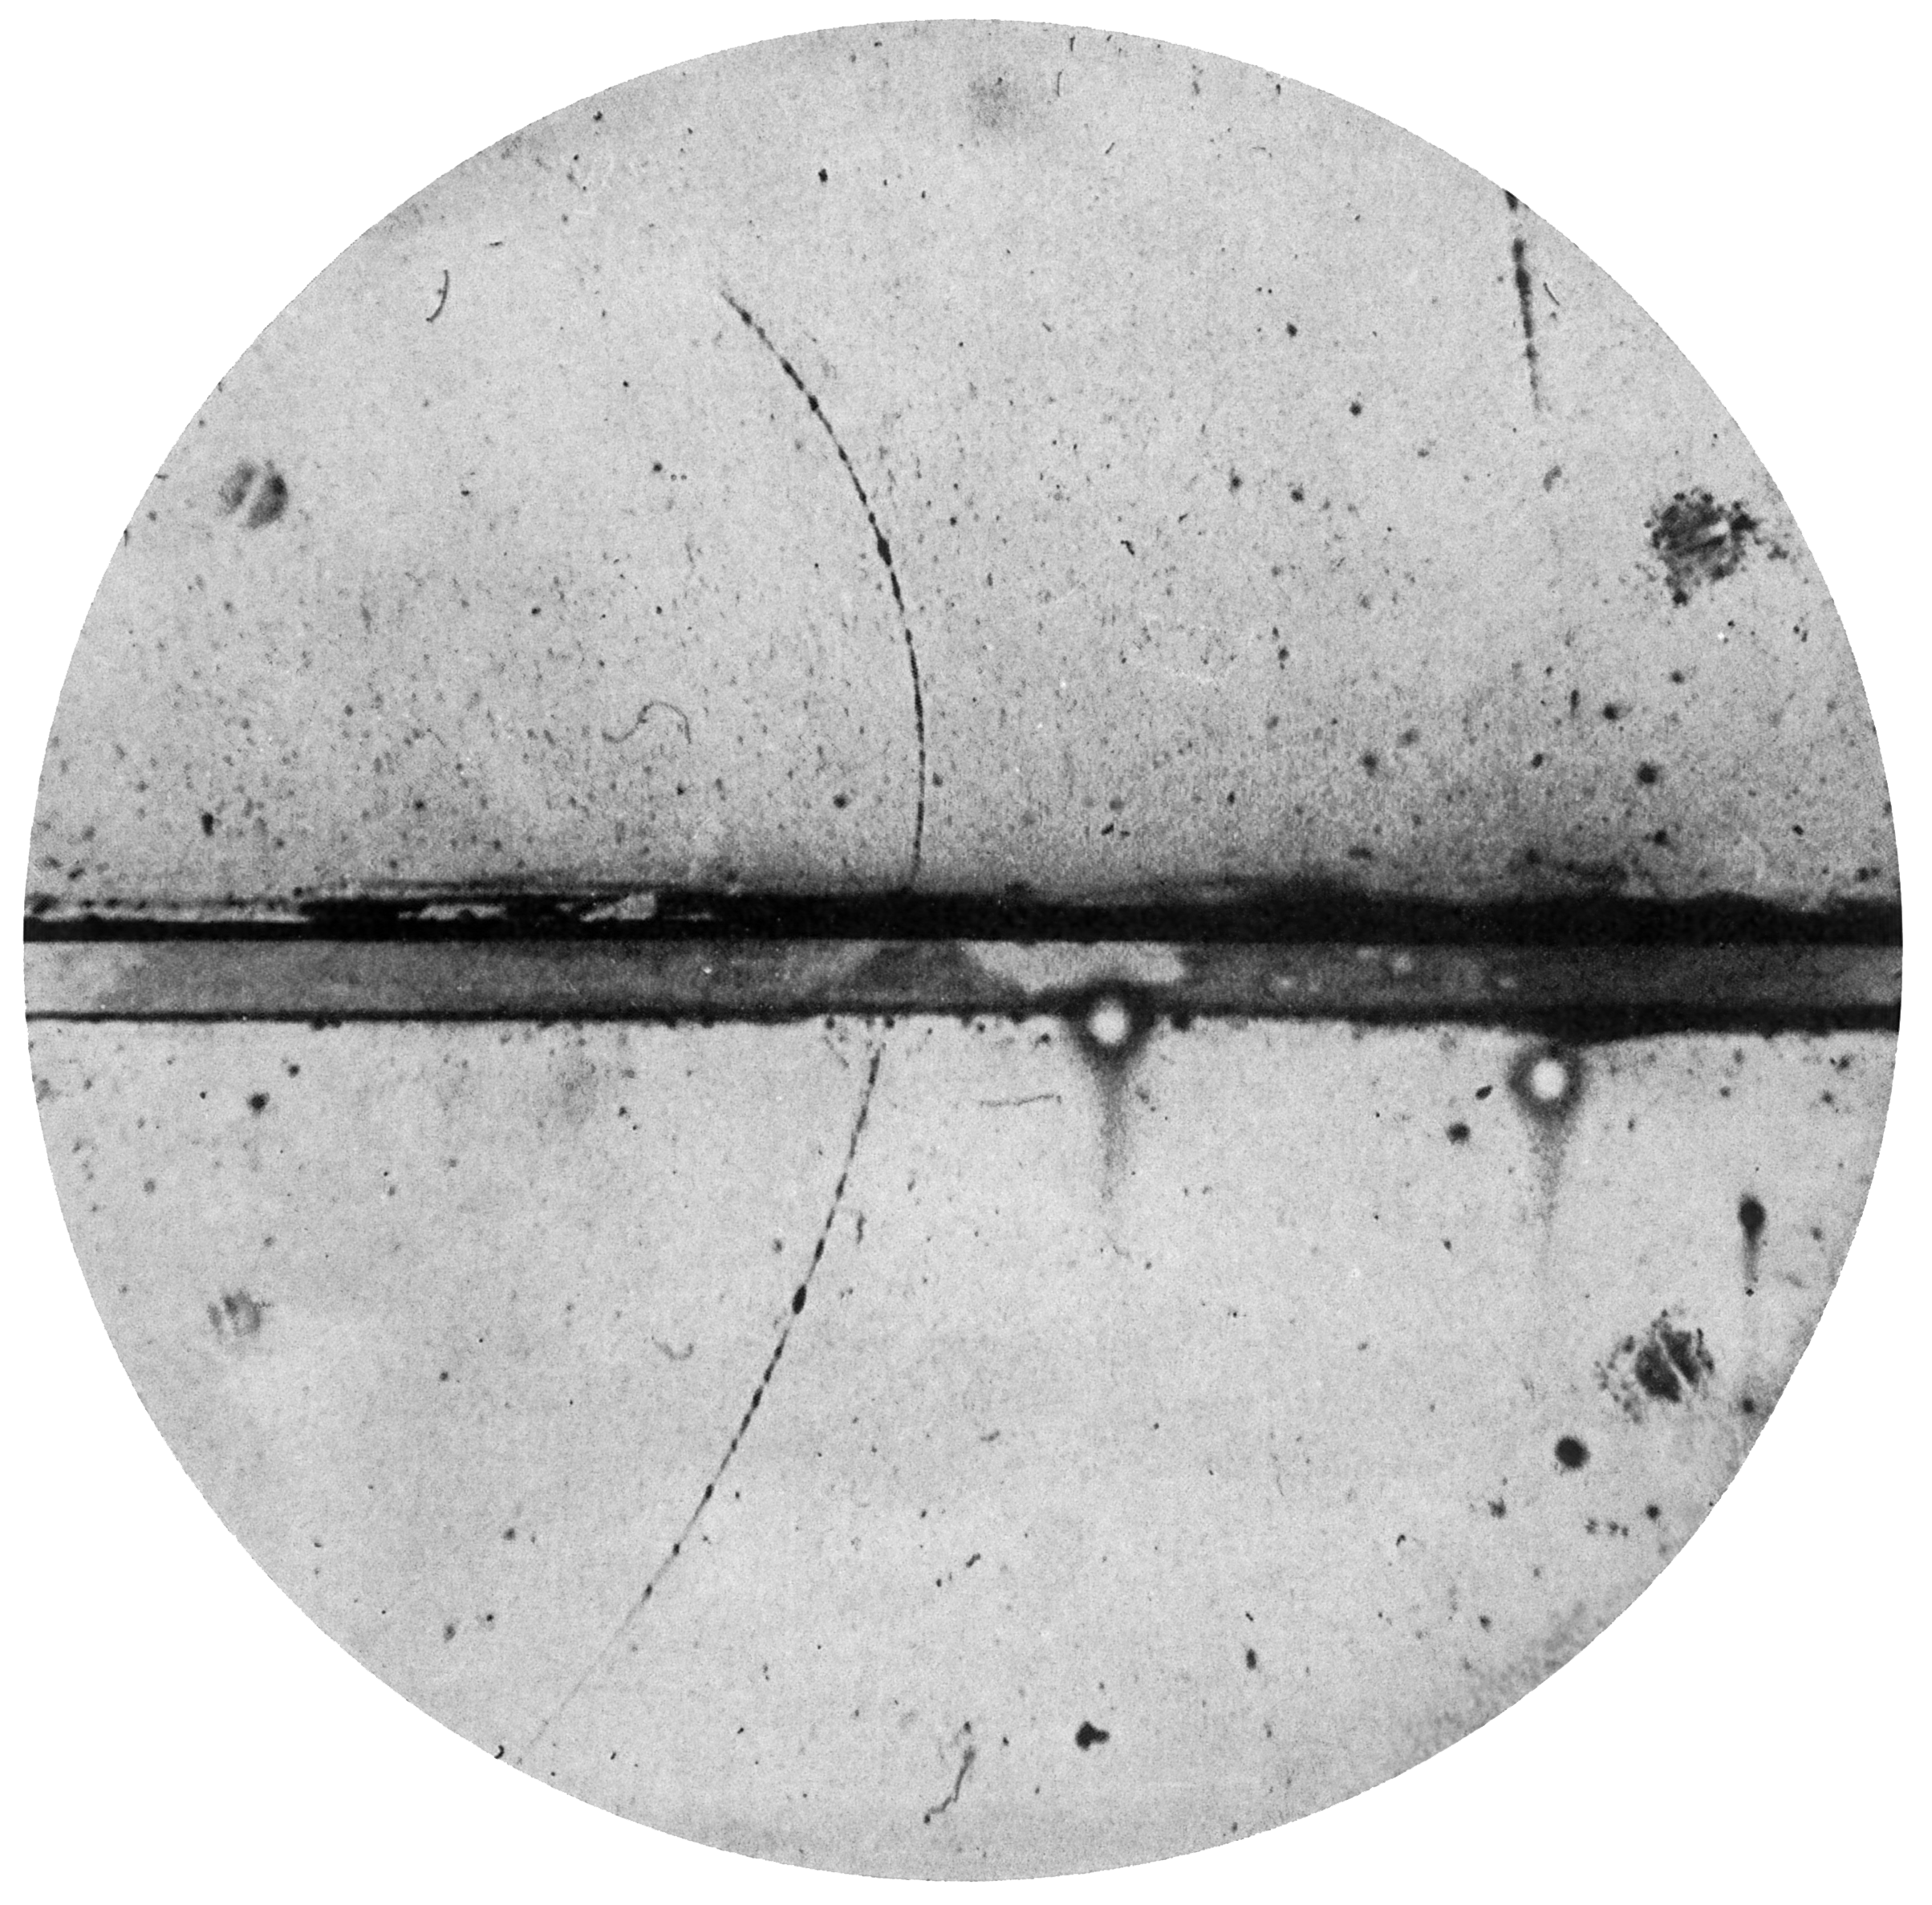
\includegraphics[width=0.55\textwidth]{figures/Part1/Field/Positron}
 \end{tabular}
 \caption{Cloud chamber photograph taken from Anderson's 1932 paper~\cite{PhysRev.43.491}. The upper chamber and the lower chamber are separated by a 6 mm lead plate. The deflection and direction of the particle's ion trail indicate that the particle is a positron.}
 \label{fig:Positron}
 \end{center}
\end{figure}

Quarks participate in all known fundamental interactions and they exist in two different types, up-type and down-type. Up-type and down-type quarks carry $+\frac{2}{3}$ and $-\frac{1}{3}$ electric charges, respectively, in units of the electron charge. For each type of quark, there exist three generations of quarks that are identical copies of each other, except their masses and flavor quantum numbers. For up-type quarks, the three generations are: i) up (u), ii) charm (c), and iii) top (t) quarks. The three generations of up-type quarks are illustrated in the first three columns of the first row in Figure~\ref{fig:Field}. For down-type quarks, the three generations are: i) down (d), ii) strange (s), and iii) bottom (b) quarks. The three generations of down-type quarks are illustrated in the first three columns of the second row in Figure~\ref{fig:Field}. Unlike leptons, which don't interact strongly, quarks carry three types of ``color'' charges: red, green, and blue, which allow them to participate in strong interactions. Strong interactions are discussed in more detail in \autoref{chap:QCD}.

With the exception of top quarks, which decay before forming bound states, quarks are only observed in bound states called ``hadrons'' as stable particles must be color neutral, and carry an integer electric charge. A quark can form two-particle bound states called ``mesons'' with another antiquark with opposite color charges. In addition to two-particle bound states, quarks can also form three- or more-particle bound states. The three-particle bound states, such as a proton (uud), are known as ``baryons''. Bound states with more than three quarks are extremely unstable with a short lifetime, such as the pentaquark recently discovered by the \ac{LHCb} experiment~\cite{LHCb:2015yax}. Because isolated quarks do not exist in nature, their existence must be inferred from the decay products of high-energy collisions. Historically, lighter quarks were observed first as the production of heavier quarks requires higher energy. For example, the existence of charm quarks was confirmed in 1974 at Brookhaven~\cite{E598:1974sol} and SLAC~\cite{SLAC-SP-017:1974ind} (illustrated in Figure~\ref{fig:JPsi}) while top quarks were only observed in 1995 at the Tevatron~\cite{CDF:1995wbb,D0:1995jca}.

\begin{figure}[tbh!]
 \begin{center}
 \begin{tabular}{c}
 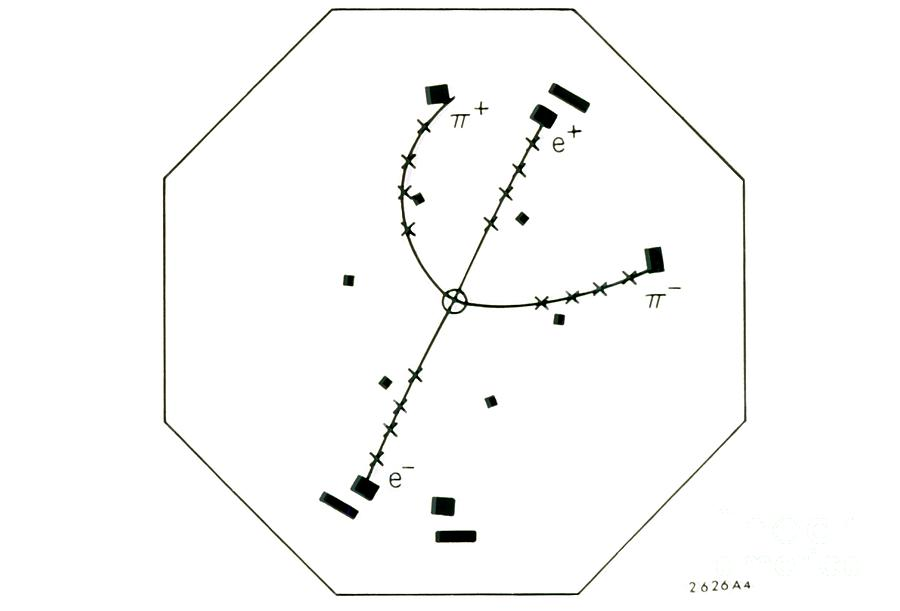
\includegraphics[width=0.7\textwidth]{figures/Part1/Field/J}
 \end{tabular}
 \caption{An example of the $\psi^{\prime}\rightarrow\psi\pi^{+}\pi^{-}$ decay recorded by the Mark I detector in the discovery of $\psi$ particle at SLAC~\cite{SLAC-SP-017:1974ind}. A new resonance around 3.1 GeV was reported by this experiment which was later confirmed to be a two-particle bound state consisting of charm and anticharm quarks.}
 \label{fig:JPsi}
 \end{center}
\end{figure}

Leptons are divided into charged leptons and neutral leptons. Charged leptons carry $-1$ electric charge while neutral leptons, as the name suggests, do not carry any electric charge. Charged leptons participate in electromagnetism and weak interactions while neutral leptons only participate in weak interactions. Similar to quarks, charged- and neutral-leptons exist in three generations, also referred to as ``flavors''. For charged leptons, the three flavors are: i) electron (e), ii) muon ($\upmu$), and iii) tau ($\uptau$). The three flavors of charged leptons are illustrated in the first three columns of the third row in Figure~\ref{fig:Field}. Neutral-leptons are known as ``neutrinos'', which are considered massless in the \ac{SM}. The three flavors of neutrinos are: i) electron neutrino ($\nu_{\textsf{e}}$), ii) muon neutrino ($\nu_{\upmu}$), and iii) tau neutrino ($\nu_{\uptau}$). The three flavors of neutral leptons are illustrated in the first three columns of the fourth row in Figure~\ref{fig:Field}.

Leptons shown in Figure~\ref{fig:Field} have definite masses created by the interaction with Higgs bosons. They are used to describe freely propagating particles of the same mass and quantum numbers, referred to as the ``mass eigenstates''. The three flavors of charged-leptons correspond exactly to their mass eigenstates, which means charged-lepton flavor is conserved in weak interactions. For neutrinos, however, their flavor eigenstates are not identical to their mass eigenstates, which allows neutrinos to oscillate between flavors as they propagate through space. The topic of fermion flavor is discussed further in \autoref{sec:Flavor}. 

The tau lepton is the only lepton that can decay into hadrons (through weak interactions), owing to its higher mass relative to other leptons. The higher mass also means more energy is needed to produce tau leptons. After a decade-long hunt, the tau lepton was eventually detected in 1974 at SLAC~\cite{Perl:1975bf}. Neutrinos only interact weakly, making it virtually impossible to detect them using any general-purpose detectors. It wasn't until the detection of tau neutrinos in 2001 by a dedicated experiment at Fermilab~\cite{DONUT:2000fbd} that all three flavors of neutrinos were experimentally confirmed. 

\section{Bosons}
\label{sec:Boson}

Bosons are named after Indian physicist Satyendra Bose, who along with Einstein, developed the foundations for Bose-Einstein statistics, which states that identical integer spin particles may occupy the same quantum state simultaneously. Elementary bosons in the \ac{SM} consist of spin-1 bosons, which behave like a vector under Lorentz transformation, and scalar bosons with a spin of 0. Vector bosons can be massive or massless and they are mediators of the fundamental forces. For example, photons are quanta of the massless vector boson field that mediates the electromagnetism between charged particles. The particle nature of photons was first demonstrated by American physicist Arthur Compton through the scattering of X-rays in 1923~\cite{PhysRev.21.483}.

The theory that describes the light-matter interaction is known as \ac{QED}, which was first formulated by Dirac in the 1920s. \ac{QED} introduces a photon field by adding two terms to the Dirac Lagrangian,

\begin{equation}
\label{eq:QED}
\mathcal{L}_{QED}=-\frac{1}{4}F_{\mu\nu}F^{\mu\nu}+i\bar{\psi}\gamma^{\mu}\partial_{\mu}\psi-m\bar{\psi}\psi-e\bar{\psi}\gamma^{\mu}A_{\mu}\psi,
\end{equation}

where the first term in Equation~\ref{eq:QED} is known as the Electromagnetic tensor, which characterizes the spacetime properties, or more formally the curvature form of the photon field. The last term in Equation~\ref{eq:QED} describes the interaction between the fermion fields, mediated by the photon field. 

However, it was soon realized that Dirac's theory was reliable only at a first order of perturbation theory. Attempts to compute high-order processes were often met with \ac{UV} divergence that were nonphysical. This problem remained unsolved for more than 20 years until the Second World War broke out, after which a procedure known as ``renormalization'' was developed independently by Japanese physicist Shinichiro Tomonaga~\cite{Tomonaga:1946zz}, American physicists Julian Schwinger~\cite{Schwinger:1948iu}, and Richard Feynman~\cite{Feynman:1950ir}. Schwinger also provided in his paper a one-loop calculation of the electron anomalous magnetic moment which matched precisely with experiments. British physicist Freeman Dyson also made important contributions by providing mathematical insights into this new technique, most notably demonstrating the equivalence between the seemingly different approaches of Feynman, Schwinger, and Tomonaga~\cite{Dyson:1949bp}. Renormalization was initially designed to systematically remove infinities that appeared in \ac{QED}. It was eventually accepted as a foundational element of quantum field theory as it ensures the validity of physics predictions at different scales. Another key feature of the \ac{QED}, known as gauge invariance, is discussed in \autoref{sec:Gauge}.

Discovered at DESY in 1979~\cite{TASSO:1979zyf}, the gluon is the second elementary boson to be observed experimentally. Like photons, gluons arise from a massless boson field with spin 1. They mediate and participate in the strong interaction as they carry color charge themselves. This property enables the self-interaction of gluons which differentiates itself from the photon. This also means that isolated gluons do not exist in nature as stable particles need to be colorless. The theory of strong interaction is known as \ac{QCD}, which is discussed further in \autoref{chap:QCD}.

Massive vector bosons exist in three types, W$^{+}$, W$^{-}$, and Z bosons. The Z boson has no electric charge while the W$^{+}$ and W$^{-}$ bosons carry the opposite electric charge and are antiparticles of each other. Together, they are also known as weak bosons as they mediate the weak interaction. Weak bosons are among the heaviest elementary particles in the \ac{SM}, behind only the top quark and the Higgs boson. The heavy mass limits the range of the weak interaction and also raises the threshold energy needed to produce them at high-energy experiments. The existence of these weak bosons was predicted by physicists in the 1960s and was confirmed nearly two decades later by experiments at \ac{CERN} in 1983~\cite{UA1:1983crd,UA2:1983tsx,UA1:1983mne,UA2:1983mlz}. The theory developed by Weinberg that provided a unified description of electromagnetism and weak interaction is discussed further in \autoref{chap:SM}.

The only known elementary boson with spin 0 is the Higgs boson, which was predicted in 1964~\cite{PhysRevLett.13.321,PhysRevLett.13.508,PhysRevLett.13.585} by six physicists including Peter Higgs whose name was given to this massive scalar boson. The Higgs boson is the second heaviest elementary particle, behind only the top quark. It has no electric charge and its associated Higgs field only interacts with other massive fields with the coupling strength proportional to the particle mass. The Higgs field provides a mechanism to generate mass for other massive elementary particles, which is discussed further in \autoref{sec:Higgs}. The high mass and lack of quantum charge make Higgs boson extremely difficult to produce. The search for this particle has been one of the longest in history, lasting over 40 years until its eventual observation in 2012 at the \ac{LHC}~\cite{ATLAS:2012yve,CMS:2012qbp}. Evidence for Higgs to two photons presented by the \ac{ATLAS} and \ac{CMS} Collaborations in 2012 is shown in Figure~\ref{fig:Hgg}.

\begin{figure}[tbh!]
 \begin{center}
 \begin{minipage}[b]{0.5\linewidth} 
 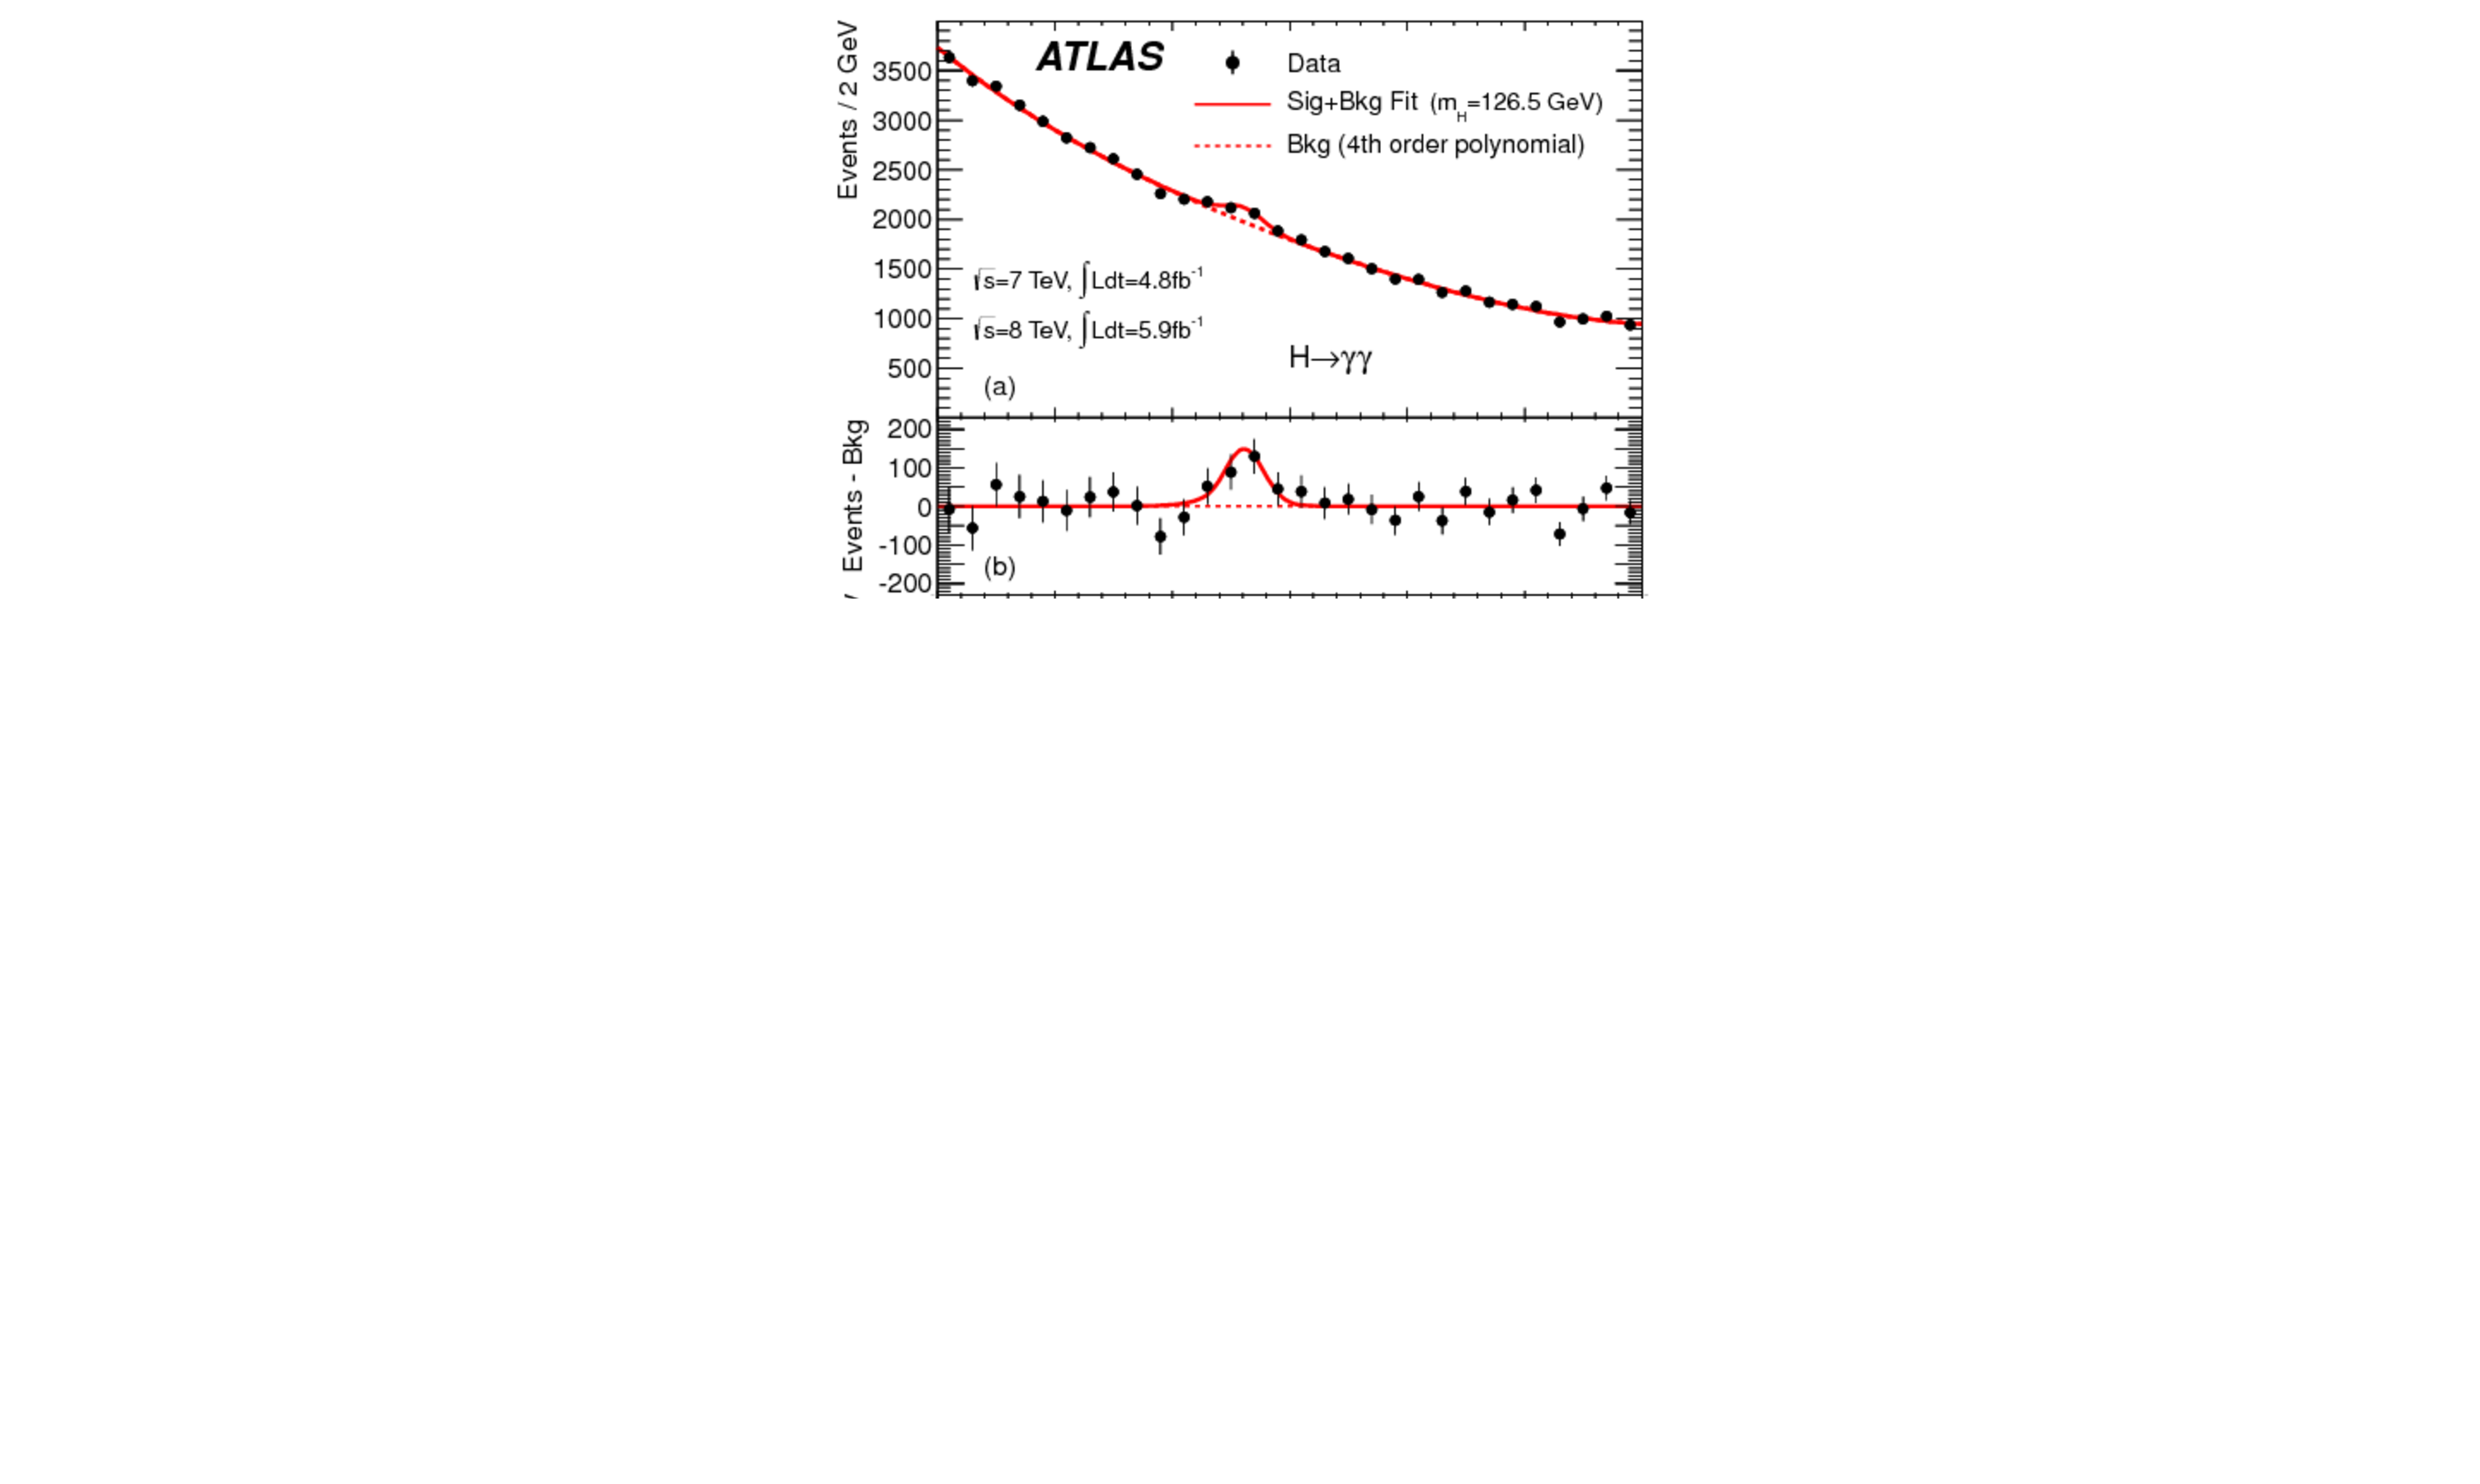
\includegraphics[width=\textwidth]{figures/Part1/Field/ATLAS} 
 \vspace{1em}
 \end{minipage}
 \hfill
 \begin{minipage}[b]{0.45\linewidth} 
 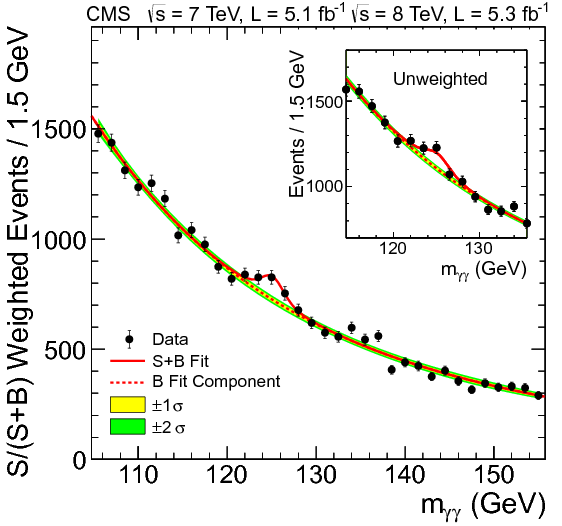
\includegraphics[width=\textwidth]{figures/Part1/Field/CMS}
 \end{minipage}
 \caption{The diphoton invariant mass distributions reported by the \ac{ATLAS}~\cite{ATLAS:2012yve} (left) and \ac{CMS}~\cite{CMS:2012qbp} (right) in their searches for the Higgs boson in 2012. The observed signal around the 125 GeV bump was consistent with the hypothesis of a new massive boson with spin 0, which was later confirmed to be the Higgs boson.}
 \label{fig:Hgg}
 \end{center}
\end{figure}
\chapter{Electroweak Theory}
\label{chap:SM}

Developed in the 1960s, the Glashow–Weinberg–Salam theory of the \ac{EW} interaction is regarded by many physicists as the cornerstone of the \ac{SM}. It successfully unified the weak interaction with electromagnetism and postulated the existence of several new particles, all of which were later confirmed by experiments. One of the most important aspects of this theory is the \ew~gauge symmetry, which is discussed in \autoref{sec:Gauge}. The \ew~ symmetry is spontaneously broken through the Higgs mechanism, which is discussed in \autoref{sec:Higgs}. Finally, flavor physics and its connection to the Yukawa interaction is discussed in \autoref{sec:Flavor}. 

\section{Gauge Theory}
\label{sec:Gauge}

Fundamental forces in the \ac{SM} are formulated under a principle known as gauge invariance, where the Lagrangian is invariant under local transformations of gauge groups. Taking \ac{QED} as an example, the local symmetry for a Dirac fermion is,

\begin{equation}
\psi\rightarrow e^{i\alpha(x)}\psi,
\end{equation}

where $\alpha(x)$ is a phase angle defined at each spacetime point, hence the name ``local transformation''. The gauge group associated with this symmetry is $U(1)_{EM}$, where the subscript is a shorthand expression for ``electromagnetism''. Under a local $U(1)_{EM}$ rotation, Equation~\ref{eq:Dirac} can be written as:

\begin{equation}
\begin{split}
\label{eq:QEDGauge}
\mathcal{L}&=-\frac{1}{4}F_{\mu\nu}F^{\mu\nu}+ie^{-i\alpha(x)}\bar{\psi}\gamma^{\mu}\partial_{\mu}e^{i\alpha(x)}\psi-m\bar{\psi}\psi-e\bar{\psi}\gamma^{\mu}(A_{\mu}+\delta A_{\mu})\psi\\
&=\mathcal{L}_{Dirac}-\bar{\psi}\gamma^{\mu}\psi\partial_{\mu}\alpha(x)-e\bar{\psi}\gamma^{\mu}\delta A_{\mu}\psi.
\end{split}
\end{equation}

The gauge invariance requires $\delta A_{\mu}=-\frac{1}{e}\partial_{\mu}\alpha(x)$. This means the photon field transforms as:

\begin{equation}
A_{\mu}\rightarrow A_{\mu}-\frac{1}{e}\partial_{\mu}\alpha(x).
\end{equation}

This behavior of the photon field under gauge transformation cancels out the gauge dependency of the free Dirac Lagrangian, which ensures the gauge invariance of the theory. Therefore, vector bosons such as photons also called gauge bosons, and the associated quantum fields are also known as gauge fields. The Dirac Lagrangian can be re-written as,

\begin{equation}
\label{eq:QEDCov}
\mathcal{L}=-\frac{1}{4}F_{\mu\nu}F^{\mu\nu}+i\bar{\psi}\gamma^{\mu}D_{\mu}\psi-m\bar{\psi}\psi,
\end{equation}

where $D_{\mu}=\partial_{\mu}+ieA_{\mu}$ is known as the gauge covariant derivative. 

The mass term associated to the photon field $\frac{1}{2}m^2A_{\mu}A^{\mu}$ is however not gauge invariant as

\begin{equation}
[A_{\mu}-\frac{1}{e}\partial_{\mu}\alpha(x)][A^{\mu}-\frac{1}{e}\partial^{\mu}\alpha(x)]\neq A_{\mu}A^{\mu}.
\end{equation}

Effectively, this means gauge bosons such as photons must be massless in a gauge invariant theory. As a consequence, a new mechanism, known as the Higgs mechanism, is needed to explain the origin of weak boson masses, which is discussed in the following chapter. 

It should be pointed out that gauge symmetry is not a symmetry of nature. The Noether currents~\cite{Noether1918} associated with local gauge symmetry do not generally correspond to physical observables. Nevertheless, its existence is necessary to regulate the redundant degree of freedom in the Lagrangian using a procedure known as gauge fixing~\cite{SCHWARTZ}. 

\ac{QED} is also known as an abelian gauge theory as the $U(1)$ group operation is commutative, meaning the order of sequential group operations does not affect the final result. Chinese physicist Chen-Ning Yang and his American colleague Robert Mills at Brookhaven first generalized the concept of gauge invariance to the non-abelian Lie group, proposing what's now known as the Yang-Mills theory in 1954~\cite{Yang:1954ek}. Shortly after this work, Yang and his colleague Tsung-Dao Lee suggested parity might be violated in the weak interaction~\cite{Lee:1956qn}, which was later confirmed by the legendary Wu experiment led by Chien-Shiung Wu~\cite{Wu:1957my}. 

Not long after the Wu experiment, physicists understood that only left-handed fermions and right-handed antifermions are involved in weak charged-current interactions. Moreover, the very existence of weak charged-current forced physicists to consider the interaction between photons and weak mediators. This led to many problems in the weak theory, for example, the exchange of photons in $s$-channel $\textsf{e}^{+}\textsf{e}^{-}\rightarrow\textsf{W}^{+}\textsf{W}^{-}$ (shown in Figure~\ref{fig:eeWW}) would lead to divergence at high energy unless there exists a neutral intermediate field that mediates the weak interaction. Hints of the weak neutral current and the interplay between electromagnetism and the weak interaction prompted the efforts by physicists to relate these two forces under the framework of Yang-Mills theory in the early 1960s. 

\begin{figure}[tbh!]
 \begin{center}
 \begin{tabular}{c}
 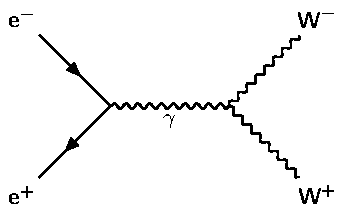
\includegraphics[width=0.6\textwidth]{figures/Part1/SM/eeWW}
 \end{tabular}
 \caption{Representative $s$ channel ee$\rightarrow$WW diagram, mediated by a massless photon field. Without a heavy neutral mediator, such a process would lead to divergence.}
 \label{fig:eeWW}
 \end{center}
\end{figure}

Since fermions with different chiral structures were understood to be treated differently by the weak interaction, it was 
imperative to apply different gauge transformations to left-handed and right-handed fermionic fields. Initial work toward unification was done by American physicist Sheldon Glashow, who proposed the \ew~symmetry in 1961~\cite{Glashow:1961tr}, where $L$ denotes left-handed fields, and Y refers to the quantum number for hypercharge. Under this framework, left-handed components of the Dirac fields are organized into $SU(2)_{L}$ doublet,

\begin{equation}
L_{L}^{j}=\begin{pmatrix}\nu^{j}\\ e^{j}\end{pmatrix}_{L}, Q_{L}^{j}=\begin{pmatrix}u^j\\d^j\end{pmatrix}_{L}, j=1, 2, 3,
\end{equation}

where $\nu^{j}$, $e^{j}$, $u^{j}$, and $d^{j}$ correspond to Dirac fields of neutrino, charged-lepton, up-type quark, and down-type quark, respectively. The right-handed components of the Dirac fields are treated as $SU(2)_{L}$ singlet: $e_{R}^{j}, u_{R}^{j}, d_{R}^{j}$, where neutrino terms are missing as only left-handed neutrinos have been observed in nature. The index $j$ in both doublets and singlets runs over the fermion generations. The left-handed doublets carry $\frac{1}{2}$ weak isospin charge, denoted by $T$. The third component of $T$, denoted by $T_3$, is $\frac{1}{2}$ for neutrinos and up-type quarks, and -$\frac{1}{2}$ for charged-leptons and down-type quarks in the $SU(2)_{L}$ doublets. All right-handed singlets carry 0 weak isospin charge, which prevents them from participating in the weak interaction. 

The \ew~symmetry introduces the following local gauge transformations:

\begin{equation}
\begin{split}
&\Psi_{L}\rightarrow\textsf{exp}[i\hat{T}^{i}\alpha^{i}(x)+i\frac{\hat{Y}}{2}\beta(x)]\Psi_{L},\\
&\Psi_{R}\rightarrow\textsf{exp}[i\frac{\hat{Y}}{2}\beta(x)]\Psi_{R},
\end{split}
\end{equation}

where $\Psi_{L}=\{L_{L}^{j},Q_{L}^{j}\}$, and $\Psi_{R}=\{e_{R}^{j}, u_{R}^{j}, d_{R}^{j}\}$. $\hat{T}^{i}$ and $\hat{Y}$ denotes generators of the $SU(2)_{L}$ and $U(1)_{Y}$ group, respectively. To preserve gauge invariance, two massless gauge fields $W_{\mu}$ and $B_{\mu}$ are introduced. The corresponding gauge covariant derivative can be written as

\begin{equation}
\label{eq:EWCov}
D_{\mu}=\partial_{\mu}-ig\hat{T}^{i}W_{\mu}^{i}-ig^{\prime}\frac{\hat{Y}}{2}B_{\mu},
\end{equation}

where $g$ and $g^{\prime}$ correspond to coupling strengths of the $SU(2)$ and $U(1)$ gauge fields, respectively. The \ew~gauge Lagrangian can therefore be written as:

\begin{equation}
\label{eq:LagGauge}
\mathcal{L}_{gauge}=-\frac{1}{2}\textsf{tr}W_{\mu\nu}W^{\mu\nu}-\frac{1}{4}B_{\mu\nu}B^{\mu\nu}+i\bar{\Psi}_{L}\gamma^{\mu}D_{\mu}\Psi_{L}+i\bar{\Psi}_{R}\gamma^{\mu}D_{\mu}\Psi_{R}
\end{equation}

A linear combination of the first and second components of gauge field $W_{\mu}^{i}$ gives rise to the weak charge-current interactions observed in experiments:

\begin{equation}
\label{eq:CC}
W^{\pm}_{\mu}=\frac{1}{\sqrt{2}}(W^{1}_{\mu}\mp W^{2}_{\mu}),
\end{equation}

while neutral-current interactions can be constructed by the remaining fields:

\begin{equation}
\label{eq:NC}
\begin{pmatrix}B_{\mu}\\W_{\mu}^{3}\end{pmatrix}=\begin{pmatrix}\cos\theta_{\omega}&-\sin\theta_{\omega}\\\sin\theta_{\omega}&\cos\theta_{\omega}\end{pmatrix}\begin{pmatrix}A_{\mu}\\Z_{\mu}\end{pmatrix},
\end{equation}

where $A_{\mu}$ and $Z_{\mu}$ correspond to the photon and Z boson, respectively, and 

\begin{equation}
\label{eq:MixAngle}
g\sin\theta_{\omega}=g^{\prime}\cos\theta_{\omega}=e.
\end{equation}

The free parameter $\theta_{\omega}$ is referred to as the weak mixing angle, or Weinberg angle, which can be measured experimentally.

The relation between electric charge, weak isospin, and hypercharge is given by the Gell-Mann-Nishijima formula~\cite{Nakano:1953zz,Gell-Mann:1956iqa}:

\begin{equation}
Q=\frac{Y}{2}+T_{3}.
\end{equation}

The preliminary version of the \ac{EW} theory developed by Glashow did not garner a huge reception initially as all gauge fields in his theory were massless due to gauge invariance, resulting in long-range forces that matched with no experimental observations. Luckily, physicists did not have to wait long as the mechanism proposed by American physicist P. W. Anderson~\cite{Anderson:1963pc} in the context of non-relativistic field theory in the following year (1962) quickly gained attention. Extending on Anderson's work, the theory of symmetry breaking and gauge boson mass generation was published by Higgs and others in 1964~\cite{PhysRevLett.13.321,PhysRevLett.13.508,PhysRevLett.13.585}, which led to the eventual completion of the \ac{EW} theory in the following years by Salam and Weinberg~\cite{Salam:1964ry,Weinberg:1967tq}.

\section{Higgs Mechanism}
\label{sec:Higgs}

The Higgs mechanism provides a way to generate a mass term for gauge bosons without explicitly breaking the gauge symmetry. The core feature of this mechanism is a $SU(2)_{L}$ doublet of complex scalar fields $\phi=\begin{psmallmatrix}\phi^{+}\\\phi^{0}\end{psmallmatrix}$, which is subject to the potential:

\begin{equation}
V(\phi)=-\mu^2(\phi^{\dagger}\phi)+\lambda(\phi^{\dagger}\phi)^2,
\end{equation}

where $\lambda$ is a real parameter that determines the Higgs quartic coupling and is required to be positive to ensure the stability of the \ac{EW} vacuum~\cite{Cabibbo:1979ay}. The parameter $\mu^2$ determines the minimum of the Higgs potential. The Lagrangian of this scalar field is written as 

\begin{equation}
\mathcal{L}_{Scalar}=(D_{\mu}\phi)^{\dagger}(D^{\mu}\phi)-V(\phi),
\end{equation}

where $D_{\mu}$ is same gauge covariant derivative shown in Equation~\ref{eq:EWCov}. The $\mathcal{L}_{Scalar}$ is invariant under \ew~gauge transformation when $\mu^2~<~0$, which corresponds to the early universe when temperature is very high, as illustrated in Figure~\ref{fig:HiggsPotential}.

\begin{figure}[tbh!]
 \begin{center}
 \begin{tabular}{c}
 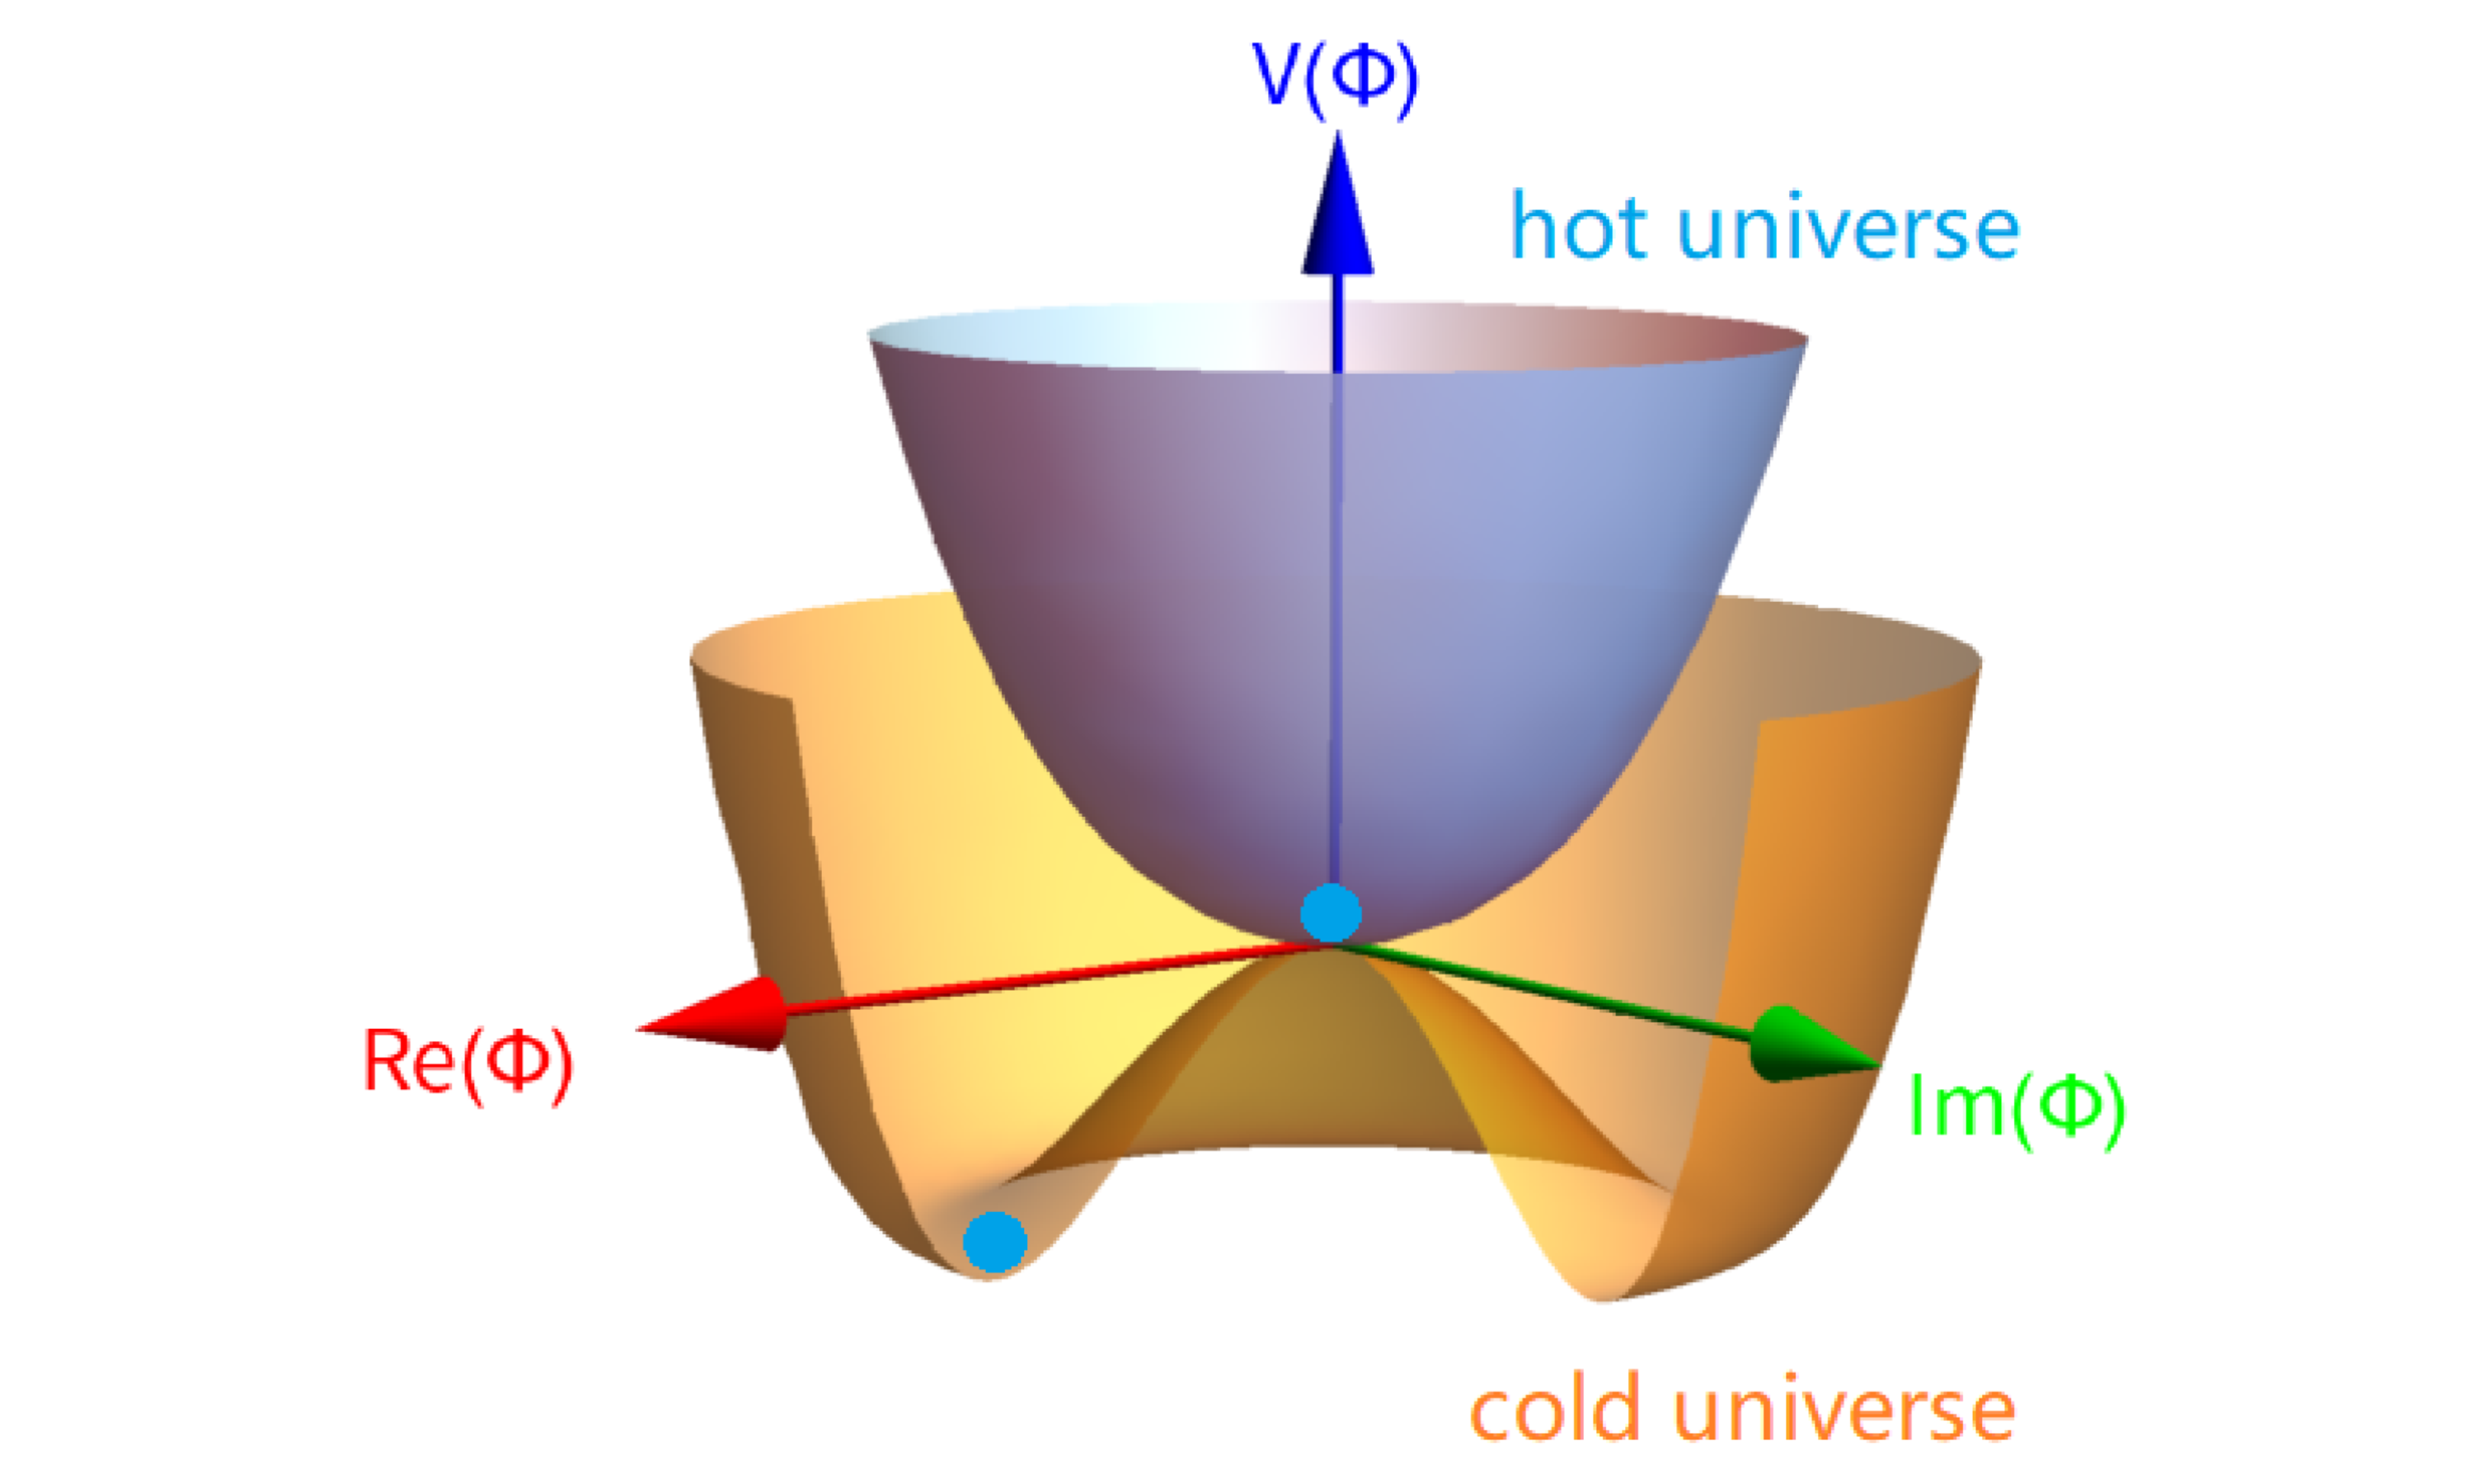
\includegraphics[width=0.7\textwidth]{figures/Part1/SM/HiggsPotential}
 \end{tabular}
 \caption{Possible shape of the Higgs potential before symmetry breaking in the hot universe (blue) and after symmetry breaking in the present universe (yellow). Adapted from~\cite{universe9040178}.}
 \label{fig:HiggsPotential}
 \end{center}
\end{figure}

Eventually, the universe cools down and $\mu^2$ becomes positive. As a consequence, an infinite number of degenerate fields arise as ground states of the potential, which corresponds to 

\begin{equation}
\phi_{min}=e^{i\varphi}\begin{pmatrix}0\\\sqrt{\mu^2/2\lambda}\end{pmatrix}\equiv\frac{e^{i\varphi}}{\sqrt{2}}\begin{pmatrix}0\\v\end{pmatrix},
\end{equation}

where $\varphi$ is the phase angle that corresponds to the choice of the degenerate field, and $v$ = 246.22 GeV~\cite{ParticleDataGroup:2022pth} is the so-called vacuum expectation value that corresponds to the physical meaning of the minimum. The ground states in this case are not invariant under \ew~symmetry. In other words, upon acquiring a vacuum expectation value by the scalar field $\phi$, the \ac{EW} symmetry will be spontaneously broken. Since the phase angle will eventually cancel out in ($\phi^{\dagger}\phi$), it is free to expand the ground-state field around the arbitrarily selected minimum $\frac{1}{\sqrt{2}}\begin{psmallmatrix}0\\v\end{psmallmatrix}$:

\begin{equation}
\phi=\frac{e^{i\hat{T}^{i}\pi^{i}(x)/v}}{\sqrt{2}}\begin{pmatrix}0\\v+h(x)\end{pmatrix},
\end{equation}

where $\hat{T}^{i}$ corresponds to the generators of the broken $SU(2)_{L}$ symmetry and $\pi^{i}(x)$ corresponds to three massless scalar bosons referred to as the Goldstone bosons~\cite{Goldstone:1962es}. The meaning of the field $h(x)$ will become clear later. The dependency on $\pi^{i}(x)$ can be removed by performing the following gauge transformation:

\begin{equation}
\phi\rightarrow\phi e^{-i\hat{T}^{i}\pi^{i}(x)/v},
\end{equation}

which corresponds to the so-called unitary gauge~\cite{Weinberg:1971fb}. Expanding the kinetic term from $\mathcal{L}_{Scalar}$,

\begin{equation}
\label{eq:ScalarKin}
(D_{\mu}\phi)^{\dagger}(D^{\mu}\phi)=\frac{1}{2}\partial_{\mu}h(x)\partial^{\mu}h(x)+(v+h(x))^2\frac{g^2}{8}[(W_{\mu}^1)^2+(W_{\mu}^1)^2+(W_{\mu}^3-\frac{g^{\prime}}{g}B_{\mu})^2].
\end{equation}

Using the relation specified in Equation~\ref{eq:CC}-\ref{eq:MixAngle}, the $v^2$ terms in Equation~\ref{eq:ScalarKin} can be rewritten as 

\begin{equation}
\begin{split}
&m_{W}^2W^{\dagger}_{\mu}W_{\mu},\\
&\frac{1}{2}m_{Z}^2Z_{\mu}Z^{\mu},
\end{split}
\end{equation}

where $m_{W}=\frac{gv}{2}$, and $m_{Z}=\frac{gv}{2\cos\theta_{\omega}}$, which corresponds to the mass of the gauge bosons W and Z, respectively. The mass of the W and Z bosons can therefore be related by $m_{Z}/m_{W}=\cos\theta_{\omega}$, which can be used to test the self-consistency of the \ac{SM}~\cite{CDF:2022hxs}. The linear combination of $v^2$ terms orthogonal to $Z_{\mu}$ cancels out and corresponds to the massless photon field:

\begin{equation}
A_{\mu}=\sin\theta_{\omega}W_{\mu}^3+\cos\theta_{\omega}B_{\mu}.
\end{equation}  

Therefore, the Z boson and photon observed at experiments can be understood as different manifestations of the same fields in the \ac{EW} theory. 

The massless gauge fields before the symmetry breaking have 2 degrees of freedom, which correspond to the two transverse polarizations. The longitudinal polarization is left empty for these massless fields because they have no rest frame when propagating in space at the speed of light. After the symmetry breaking, the $W^{\pm}_{\mu}/Z_{\mu}$ gauge fields acquire masses, which also means that they acquire longitudinal polarizations. Therefore, it can be said that the three ``would-be'' Goldstone bosons are ``eaten'' by the three gauge bosons, becoming their longitudinal components.

The remaining scalar field $h(x)$ gives rise to the only elementary scalar boson in the \ac{SM}, known as the Higgs boson. Except two mass terms for W and Z bosons, and a constant term 

\begin{equation}
\frac{1}{2}\mu^2v^2-\frac{\lambda}{2}v^4=\frac{1}{2}v^4
\end{equation}

coming from the potential, all terms in $\mathcal{L}_{Scalar}$ are related to the $h(x)$ field. They can be collected together as $\mathcal{L}_{Higgs}$:

\begin{equation}
\label{eq:LHiggs}
\begin{split}
\mathcal{L}_{Higgs}=&\frac{1}{2}\partial_{\mu}h(x)\partial^{\mu}h(x)-\frac{1}{2}m_{H}^2h(x)^2-\frac{1}{2v}m_{H}^2h(x)^3-\frac{1}{8v^2}m_{H}^2h(x)^4\\
&+[\frac{2}{v}h(x)+\frac{1}{v^2}h(x)^2](m_{W}^2W_{\mu}^{\dagger}W^{\mu}+\frac{1}{2}m_{Z}^2Z_{\mu}Z^{\mu}),
\end{split}
\end{equation}

where $m_{H}=\sqrt{2\lambda}v$. The third and fourth terms on the first line of Equation~\ref{eq:LHiggs} correspond to the Higgs triple and quartic couplings, respectively, and they come from the potential term in $\mathcal{L}_{Scalar}$. The terms on the second line of Equation~\ref{eq:LHiggs} correspond to the Higgs-Gauge boson couplings, and they come from the kinetic terms in $\mathcal{L}_{Scalar}$. The strength of these coupling is proportional to the masses of the gauge bosons. 

\section{Yukawa Interaction and Flavor Sector}
\label{sec:Flavor}

Adding Dirac mass terms $-m\bar{\psi}\psi=-m(\bar{\psi}_{L}\psi_{R}+\bar{\psi}_{R}\psi_{L})$ to the \ac{EW} theory directly will not be allowed, because they explicitly break the \ew~symmetry. Instead, the origin of the fermion masses is explained by the interaction between fermionic fields and the scalar field introduced earlier, which was first pointed out by Weinberg in his famous 1967 paper~\cite{Weinberg:1967tq}. This interaction is described by the $\mathcal{L}_{Yukawa}$ written as:

\begin{equation}
\label{eq:Yukawa}
\mathcal{L}_{Yukawa}=-(Y_{u})_{ij}\bar{Q}_{L}^{i}u_{R}^{j}\tilde{\phi}-(Y_{d})_{ij}\bar{Q}_{L}^{i}d_{R}^{j}\phi-(Y_{e})_{ij}\bar{L}_{L}^{i}e_{R}^{j}\phi + h.c.,
\end{equation}

where $Y_{f}~(f=u,d,e)$ are complex 3$\times$3 matrices, $\tilde{\phi}=i\sigma_{2}\phi^{*}$ with $\sigma_{2}$ being the second Pauli matrix. Indices i and j run over fermion generations. After the \ac{EW}~symmetry breaking, the $\mathcal{L}_{Yukawa}$ in unitary gauge becomes:

\begin{equation}
\mathcal{L}_{Yukawa}=-\frac{1}{\sqrt{2}}(v+h(x))[(Y_{u})_{ij}\bar{u}_{L}^{i}u_{R}^{j}-(Y_{d})_{ij}\bar{d}_{L}^{i}d_{R}^{j}-(Y_{e})_{ij}\bar{e}_{L}^{i}e_{R}^{j}] + h.c.,
\end{equation}

which can be rewritten as:

\begin{equation}
\mathcal{L}_{Yukawa}=-(1+\frac{h(x)}{v})[(m_{u})_{ij}\bar{u}_{L}^{i}u_{R}^{j}+(m_{d})_{ij}\bar{d}_{L}^{i}d_{R}^{j}+(m_{e})_{ij}\bar{e}_{L}^{i}e_{R}^{j}] + h.c.,
\end{equation}

where $m_f=\frac{v}{\sqrt{2}}Y_{f}~(f=u,d,e)$ is known as the fermion mass matrices. The mass matrices can be diagonalized by unitary rotations:

\begin{equation}
m_{f}=V_{f}\hat{m}_{f}W^{\dagger}_{f}~(f=u,d,e),
\end{equation}

where $\hat{m}_{f}$ are the diagonalized mass matrices. The mass term becomes:

\begin{equation}
\mathcal{L}_{mass}=-(\bar{u}_{L}V_{u}\hat{m}_{u}W_{u}^{\dagger}u_{R}+\bar{d}_{L}V_{d}\hat{m}_{d}W^{\dagger}_{d}d_{R}+\bar{e}_{L}V_{e}\hat{m}_{e}W_{e}^{\dagger}e_{R}) + h.c.
\end{equation}

Going to the so called ``mass basis'' with $u_{L}\rightarrow V_{u}u_{L}$, $u_{R}\rightarrow W_{u}u_{R}$, ...

\begin{equation}
\mathcal{L}_{mass}=-(\bar{u}_{L}\hat{m}_{u}u_{R}+\bar{d}_{L}\hat{m}_{d}d_{R}+\bar{e}_{L}\hat{m}_{e}e_{R}) + h.c.,
\end{equation}

where the diagonal elements of $\hat{m}_{f}~(f=u,d,e)$ corresponds to the Dirac mass observed in experiments. 

On the other hand, these basis transformations will affect the charged-current interactions contained in the third term of $\mathcal{L}_{gauge}$ (Equation~\ref{eq:LagGauge}):

\begin{equation}
\label{eq:LCC}
\mathcal{L}_{cc}=-\frac{g}{\sqrt{2}}[\bar{u}_{L}\gamma^{\mu}(V_{u}^{\dagger}V_{d})d_{L}+\bar{\nu}_{L}\gamma^{\mu}(V_{\nu}^{\dagger}V_{e})e_{L}]W_{\mu}^{+} + h.c, 
\end{equation}

where fermion flavor indices are suppressed, $V_{u}^{\dagger}V_{d}$ is known as the \ac{CKM} matrix~\cite{Cabibbo:1963yz,Kobayashi:1973fv}, and $V_{\nu}^{\dagger}V_{e}$ is known as the \ac{PMNS} matrix~\cite{Pontecorvo:1957cp,Maki:1962mu}. 

The \ac{CKM} matrix is a 3$\times$3 complex unitary matrix and is generally not diagonal as $V_{u}\neq V_{d}$. This enables quark flavor mixings in the charged-current interactions. For leptons, however, it is free to choose $V_{\nu}=V_{e}$ as there is no neutrino term in the $\mathcal{L}_{Yukawa}$. Therefore, the \ac{PMNS} matrix only contains diagonal elements \ac{SM} which imply the conservation of the lepton flavors.  

Looking closely at the charged-current interactions in the lepton sector:

\begin{equation}
\label{eq:LepCC}
\begin{split}
\mathcal{L}_{cc}^{lep}&=-\frac{g}{\sqrt{2}}[(\bar{\nu}_{L}^{e},\bar{\nu}_{L}^{\mu},\bar{\nu}^{\tau}_{L})\gamma^{\mu}\begin{psmallmatrix}1&0&0\\0&1&0\\0&0&1\end{psmallmatrix}(e_{L},\mu_{L},\tau_{L})^{T}]W_{\mu}^{+} + h.c.\\
&=-\frac{g}{\sqrt{2}}(\bar{\nu}_{L}^{e}\gamma^{\mu}e_{L}+\bar{\nu}_{L}^{\mu}\gamma^{\mu}\mu_{L}+\bar{\nu}_{L}^{\tau}\gamma^{\mu}\tau_{L})W^{+}_{\mu} + h.c.
\end{split}
\end{equation}

The Lagrangian is invariant under three independent global $U(1)$ symmetry, namely $U(1)_{e}\bigotimes\\U(1)_{\mu}\bigotimes U(1)_{\tau}$, which correspond to the conserved charges: family numbers of three flavors. Moreover, since the coupling strength is the same across lepton generations in Equation~\ref{eq:LepCC}, it implies that leptons of different flavors are treated equally by the weak interactions. This is the principle known as the lepton flavor universality.

It should be pointed out that the global $U(1)_{e}\bigotimes U(1)_{\mu}\bigotimes U(1)_{\tau}$ symmetry is accidental because it does not arrive by construction. Instead, it is driven by the field content of the \ac{SM}, namely the absence of right-handed neutrinos. 
\chapter{Quantum Chromodynamics}
\label{chap:QCD}

The strong interaction is the fundamental force responsible for binding quarks together into hadrons. It is described by \ac{QCD} which is a gauge theory based on $SU(3)_{C}$ symmetry. One of the key features of \ac{QCD} is the phenomenon known as asymptotic freedom, namely strong force weakens at shorter distances. This property differentiates the strong force from all three other fundamental forces. A brief description of the formulation of \ac{QCD} is given in \autoref{sec:QCD}. Asymptotic freedom predicts that the strong coupling constant, denoted by $\alpha_{S}$, is small at short distances, which allows for perturbative expansion of the probability amplitude. However, the expansion parameter $\alpha_{S}$ at long distances becomes too large and the predictions are therefore no longer reliable. Techniques developed to model \ac{QCD} phenomenon in this regime are collectively known as nonperturbative-\ac{QCD}, which is discussed in \autoref{sec:Collision}.

\section{Formulation of QCD}
\label{sec:QCD}

The theory of strong interaction began taking its current form in 1964 when the quark model was independently proposed by American physicists George Zweig~\cite{Zweig:1964ruk} and his Ph.D. advisor Murray Gell-Mann~\cite{Gell-Mann:1964ewy}. The original objective of this model was to explain the spectrum of new hadrons discovered at a rapid speed at the time. In this early version, mesons and baryons were viewed as composite objects formed by spin-$\frac{1}{2}$ particles, named ``quarks'' by Gell-Mann and ``aces'' by Zweig. They came with several quantum charges and three different flavors: $u$, $d$, $s$. The strange quarks in this model had a higher mass, which explained the mass differences between different baryons and mesons.

This model was successful in explaining why protons of the same charge were bound together -- they were bound states of more fundamental particles affected by the strong interactions. However, gaps still existed in this model, mostly notably the tension with Fermi-Dirac statistics. It was indicated by this model that the wave function for $\mathrm{\Omega^{-}}$ (sss) should be symmetrical in the interchange of strange quarks. However, the wave function must be antisymmetric because quarks had half spins in this model. Gell-Mann and his collaborations were able to resolve this problem in the early 1970s by introducing color charges~\cite{Fritzsch:1973pi}. Under this updated framework, each flavor of quark should come with three colors, namely red, green, and blue. The wave functions of hadrons were assumed to be singlets of the gauge group $SU(3)_{C}$. For example, the wave function for $\mathrm{\Omega^{-}}$ baryon can be represented as,

\begin{equation}
(sss)\rightarrow(s_{r}s_{g}s_{b}-s_{g}s_{r}s_{b}+s_{b}s_{r}s_{g}-s_{r}s_{b}s_{g}+s_{g}s_{b}s_{r}-s_{b}s_{g}s_{r}),
\end{equation}

which restored the Fermi-Dirac statistics.  

The force mediators in this theory, known as ``gluons'', are massless vector bosons analogous to photons. They are electrically neutral but carry color charges, which enables the gluon-gluon self-interactions. The dynamics of gluon-gluon and quark-gluon interactions are described by the \ac{QCD} Lagrangian in the following form:

\begin{equation}
\mathcal{L}_{QCD}=-\frac{1}{2}\textsf{tr}G_{\mu\nu}G^{\mu\nu}+\bar{Q}(i\gamma^{\mu}D_{\mu}-m)Q,
\end{equation}

where $Q$ represents colour triplets quark fields $(Q_{r},Q_{g},Q_{b})^{T}$ of the $SU(3)_{C}$ group that run over six different flavors, $m$ corresponds to the mass of quarks. $G_{\mu\nu}$ is known as the gluon field strength tensor given by

\begin{equation}
\label{eq:G}
G_{\mu\nu}^{a}=\partial_{\mu}A_{\nu}^{a}-\partial_{\nu}A_{\mu}^{a}+g_{S}f^{abc}A_{\mu}^{b}A_{\nu}^{c},
\end{equation}

where $g_{S}$ corresponds to the strength of the gauge coupling. The strong coupling constant is also defined as $\alpha_{S}=\frac{g_{S}^2}{4\pi}$, which is analogous to the fine structure constant in \ac{QED}. $t_{a}$ are eight generators of the $SU(3)_{C}$ group, and $A^{a}_{\mu}$ represent eight gauge fields correspond to eight gluons. $f^{abc}$ is the structure constant defined by $[t^{a},t^{b}]=if^{abc}t^{c}$. $D_{\mu}$ is the $SU(3)_{C}$ gauge covariant derivative expresses as:

\begin{equation}
D_{\mu}=\partial_{\mu}-ig_{S}t_{a}A^{a}_{\mu}.
\end{equation}

The non-abelian structure of the $SU(3)_{C}$ group implies that the third term in Equation~\ref{eq:G} is nonzero as $SU(3)_{C}$ generators do not commute with each other. This leads to the trilinear and quartic gluon self-interactions when expanding the kinetic (first) term of the \ac{QCD} Lagrangian. Feynman diagrams for these gluon self-interactions are shown in Figure~\ref{fig:gluonself}.

\begin{figure}[tbh!]
 \begin{center}
 \begin{tabular}{cc}
 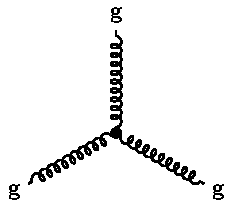
\includegraphics[width=0.45\textwidth]{figures/Part1/QCD/QCD3}&
 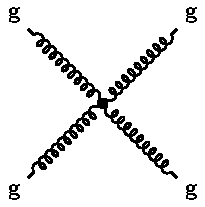
\includegraphics[width=0.4\textwidth]{figures/Part1/QCD/QCD4}\\
 \end{tabular}
 \caption{Feynman diagrams correspond to the trilinear (left) and quartic (right) gluon self-interactions.}
 \label{fig:gluonself}
 \end{center}
\end{figure}

In parallel to the development of the quark model, Feynman proposed a model to explain the behavior of deep inelastic scatterings~\cite{Feynman:1969wa}. In this model, Feynman postulated that protons are made of point-like constituents called ``partons'', and they behave like free particles at high momentum transfer. Since the de Broglie wavelength~\cite{deBroglie:1924ldk} is given by 

\begin{equation}
\lambda=\frac{h}{p}, 
\end{equation}

a high momentum transfer corresponds to a smaller wavelength and consequently better experimental resolution at the distance scale. The parton model was an immediate success as it was able to predict the short distance ``Bjorken scaling'' effects of the strong interaction at a very good precision~\cite{Bjorken:1969ja}. Despite the success at describing experimental data, the parton model was still viewed as a phenomenological approximation as Feynman provided no microscopic description of the strong interactions. It was later recognized that partons were matched to quarks, anti-quarks, and gluons within the nucleons.

Two years after Dutch physicist Gerard 't Hooft showed that non-abelian gauge theories were renormalizable~\cite{tHooft:1971akt}, major breakthrough came in 1973 when American physicists H. D. Politzer, David Gross, and Frank Wilczek~\cite{Gross:1973id,Politzer:1973fx} investigated the scale dependency of the strong coupling const $\alpha_{S}$. 't Hooft also arrived at similar results himself sometime earlier but he didn't publish his work. At one-loop precision, the $\alpha_{S}(\mu^2)$ is given by:

\begin{equation}
\label{eq:af}
\alpha_{S}(\mu^2)=\frac{\alpha_{S}(\mu_{R}^2)}{1+\beta_{0}\alpha_{S}(\mu_{R}^2)\textsf{ln}(\frac{\mu^2}{\mu_{R}^2})}
\end{equation}

where $\mu$ is the energy scale, $\mu_{R}$ is known as the renormalization scale, which corresponds to the initial energy scale at which $\alpha_{S}$ is evaluated. $\beta_{0}=(33-2n_{f})/12\pi$ is a constant that depends on the number of quark flavors that can be considered massless. Even though the strong coupling constant can not be predicted from the first principle, Equation~\ref{eq:af} allows physicists to predict its value at an energy scale $\mu$ using its measured value at a different scale $\mu_{R}$.

Equation~\ref{eq:af} also reveals that when $n_{f}~<16$, the strength of the strong coupling decreases as energy increases. In other words, quarks and gluons behave like free particles at very short distances. The discovery of this property, known as ``asymptotic freedom'', by Politzer, Gross, and Wilczek brought the \ac{SM} to its current formulation. Since then it has withstood the test of numerous measurements conducted at various experiments across a wide range of energy spectrum. A summary of recent measurements of $\alpha_{S}$ is given in Figure~\ref{fig:alphaS}.

\begin{figure}[tbh!]
 \begin{center}
 \begin{tabular}{c}
 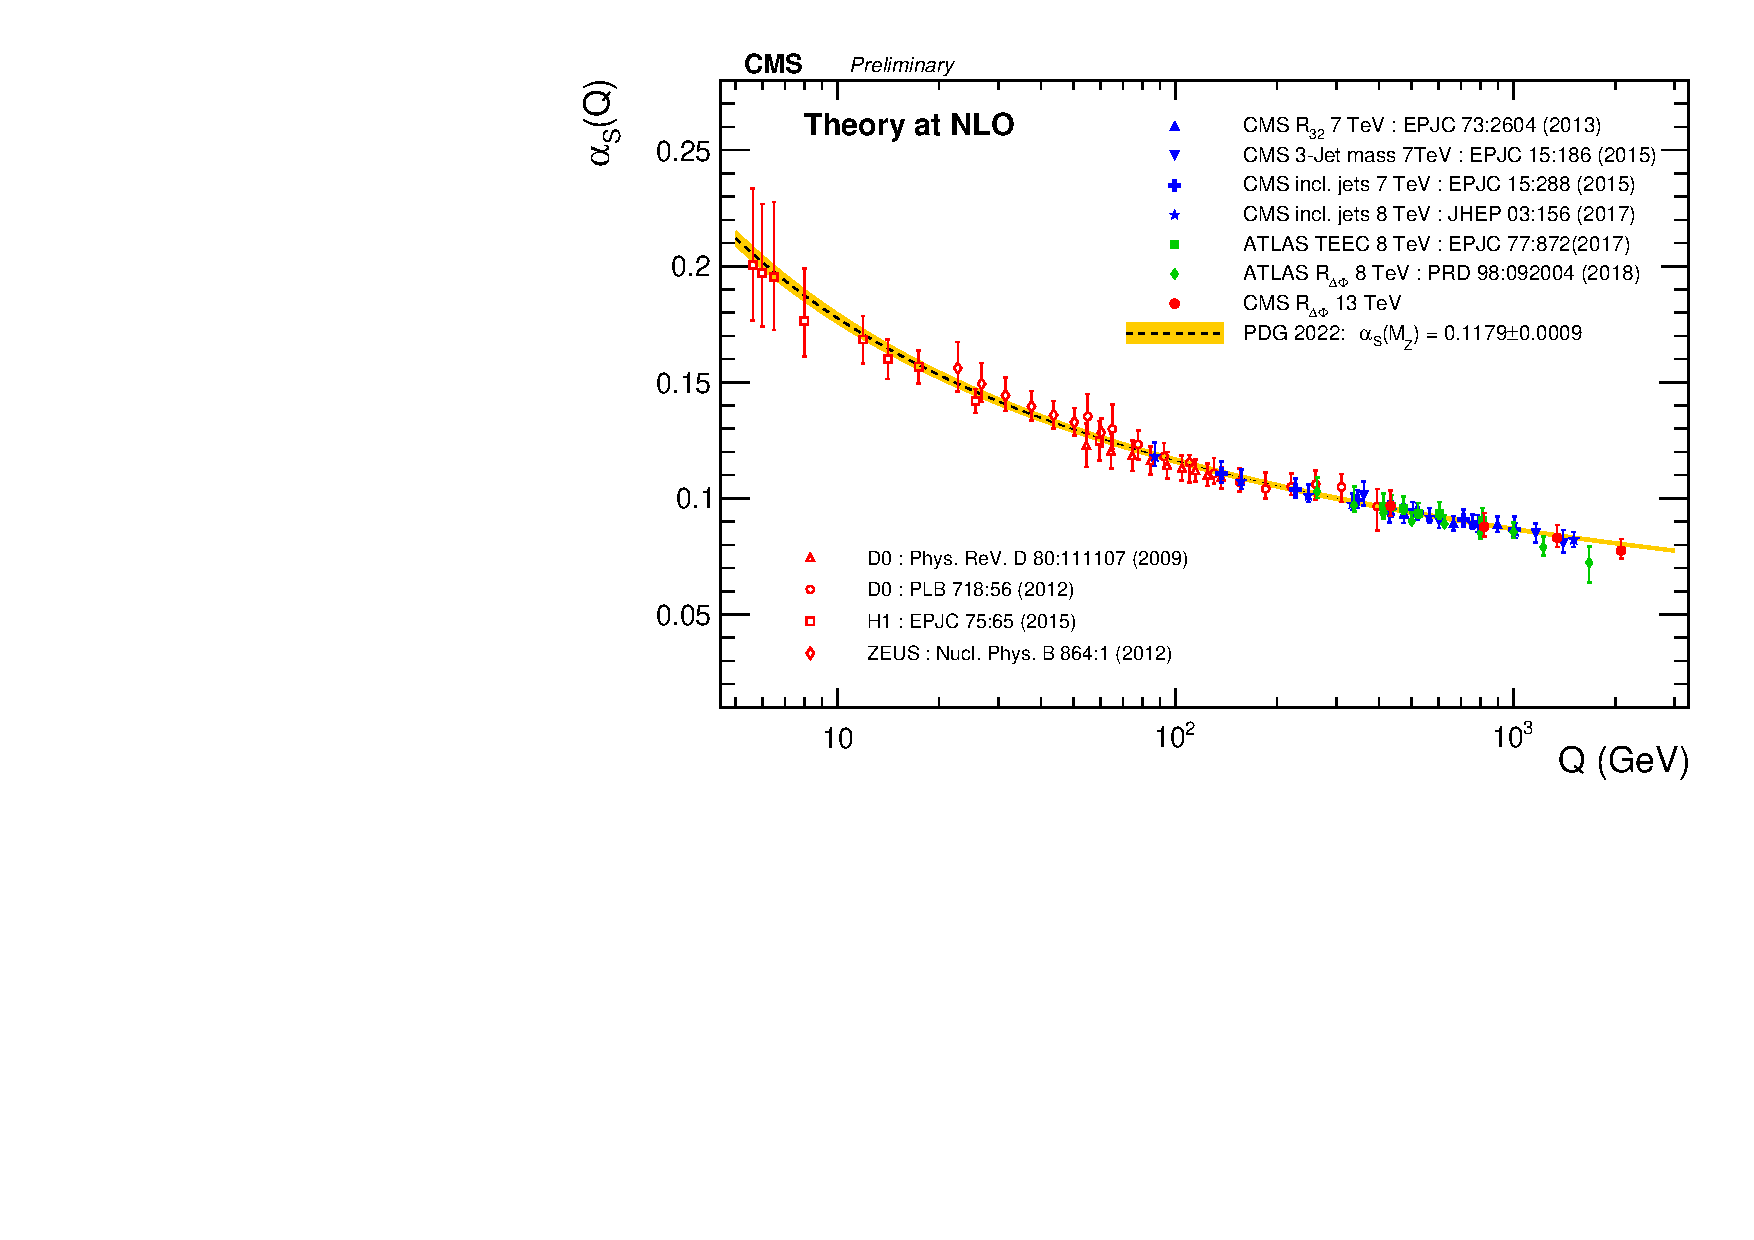
\includegraphics[width=0.8\textwidth]{figures/Part1/QCD/alphaS}
 \end{tabular}
 \caption{The strong coupling constant $\alpha_{S}$ as a function of energy scale $Q$. Measurements done by \ac{CMS}, \ac{ATLAS}, and other experiments were shown in points with uncertainty bars. Theoretical predictions based on the renormalization group equation are shown in the dashed line.~\cite{cms:twiki}}
 \label{fig:alphaS}
 \end{center}
\end{figure}

\section{Nonperturbative QCD and Hadron Collisions}
\label{sec:Collision}

Perturbation theory is by far the best-developed tool for calculating scattering cross-sections from the first principle. Despite being very successful, its predicting power becomes increasingly worse as the expansion parameter grows larger. As discussed earlier, the strong interaction grows stronger very rapidly at low energy which invalidates the perturbative expansions of parameter $\alpha_{S}$. The transition from perturbative \ac{QCD} regime to nonperturbative \ac{QCD} regime is illustrated in Figure~\ref{fig:pQCD}. The energy scales at which $\alpha_{S}$ diverges is known as $\mathrm{\Lambda}_{QCD}$, which is roughly $\mathcal{O}$(300 MeV)~\cite{Deur:2016tte}.

\begin{figure}[tbh!]
 \begin{center}
 \begin{tabular}{c}
 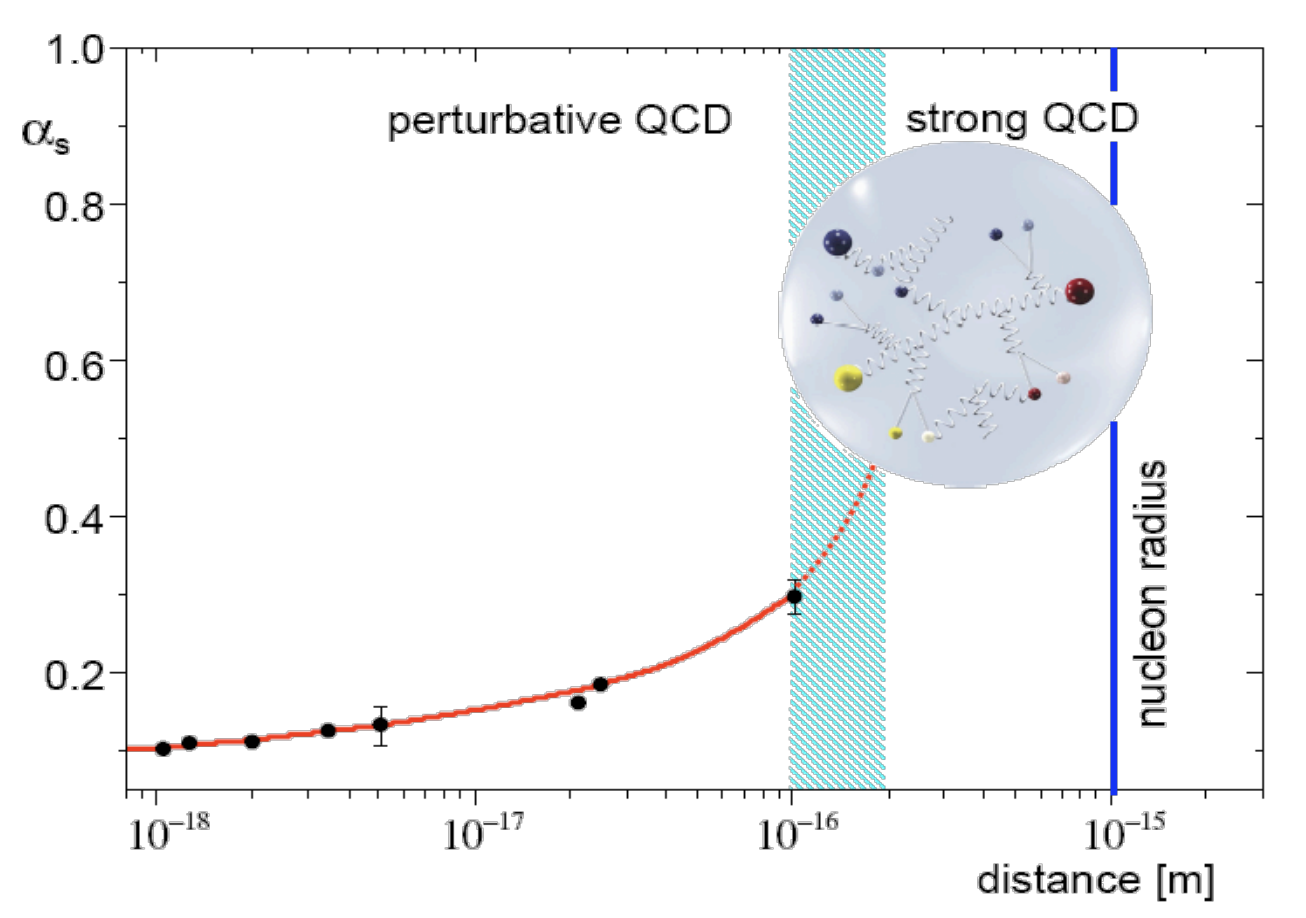
\includegraphics[width=0.7\textwidth]{figures/Part1/QCD/pQCD}
 \end{tabular}
 \caption{The strong coupling constant $\alpha_{S}$ as a function of distance scale. Experimental determinations are shown in filled points while theoretical predictions are shown in the red line. The dashed blue band separates the regime where the perturbative approach is still valid from the regime where the perturbative approach is no longer valid.~\cite{Messchendorp:2013ysj}}
 \label{fig:pQCD}
 \end{center}
\end{figure}

The high energy hadron collisions involve phenomena occurring on a wide range of distances or energy scales. The process that carries the highest momentum transfer in a collision event, referred to as ``hard scattering'', typically involves short-distance quark-gluon interactions where production cross-sections calculated by perturbative \ac{QCD} are still valid. It is therefore critically important to separate the hard scattering from those long-distance effects in order to apply the perturbative \ac{QCD} in any cross-section calculations. This is achieved through the so-called \ac{QCD} ``factorization theorem''~\cite{Collins:1989gx} whereby scattering cross-sections are decomposed as the product of several ``factors''. Each of these factors involves phenomena occurring on a single distance scale. An illustration of the factorization is shown in Figure~\ref{fig:factorization}.

\begin{figure}[tbh!]
 \begin{center}
 \begin{tabular}{c}
 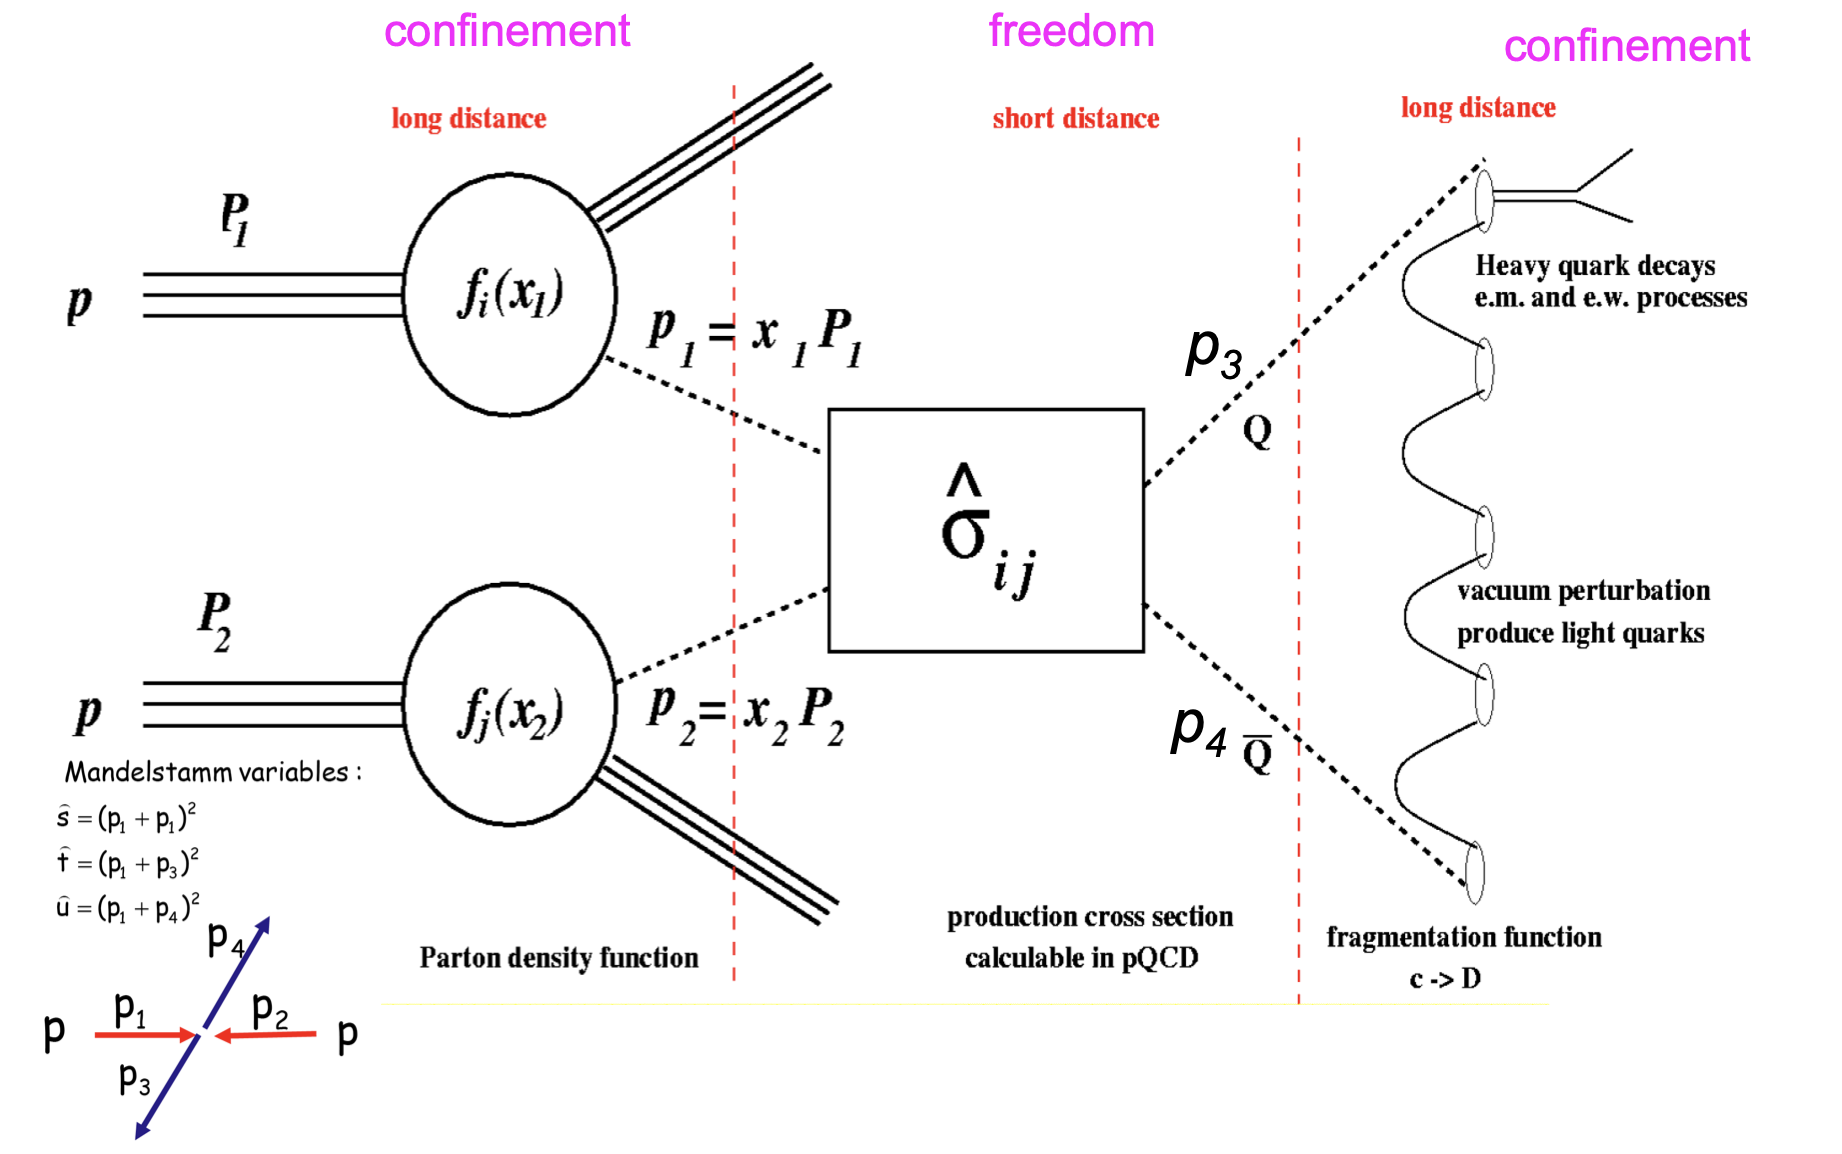
\includegraphics[width=0.9\textwidth]{figures/Part1/QCD/factorization}
 \end{tabular}
 \caption{Illustration of the physics of proton-proton collisions. The two incoming protons are shown on the left. The \ac{PDF} characterizes the properties of the two partons that participate in hard interaction. The short-distance physics is handled by the perturbative \ac{QCD} which is represented with the rectangular box. The outgoing partons undergoes hadronization which is described by the \ac{FF}.~\cite{Huston:fact}}
 \label{fig:factorization}
 \end{center}
\end{figure}

Protons are made of two up quarks and one down quark, known as the ``valence quarks''. Since the total mass of the three valence quarks is much smaller than the mass of a proton, most of the proton mass manifests as strong interactions within the nucleons. The mediators of these interactions -- the gluons can also spawn a pair of quark and anti-quark, forming part of the proton internal structure known as the ``proton sea''. Therefore, it is possible for strange, charm, or even bottom quarks to initiate a hard scattering, and the three-quark view of the proton is largely ineffective in the context of hadron collisions. Moreover, before the initial state of the hard scattering reveals itself, the quarks and gluons inside the proton maintain a relatively large distance between each other, exchanging largely nonperturbative effects. This makes it virtually impossible to predict, from the first principle, the structure of the proton before the hard scattering. 

A phenomenological approach, inspired by Feynman's parton model, is used to describe the proton's internal structure. Under this approach, protons are seen as streams of quarks and gluons, collectively known as partons. These partons are considered collinear with the proton movement and each carries a fraction of the total proton momentum. The probability of a specific parton $a$ that carries $x_{a}$ fraction of the proton momentum is given by the \ac{PDF} $F_{a}(x,\mu_{F}^2)$ where $\mu_{F}$ is the energy scale that defines the boundary between the short-distance and long-distance dynamics, known as the factorization scale. The cross-section for the production of a generic hadron or hadrons $X$ from proton-proton collisions is given by the \ac{LHC} ``master formula'':

\begin{equation}
\label{eq:master}
\sigma_{pp\rightarrow X}=\sum_{a,b}\int_{0}^{1}dx_{1}dx_{2}dzF_{a}(x_{1},\mu_{F}^2)F_{b}(x_{2},\mu_{F}^2)\hat{\sigma}_{ab\rightarrow k}(\mu_{R}^2,\mu_{F}^2)D_{k\rightarrow X}(z,\mu_{F}^2).
\end{equation} 

As \acp{PDF} only describe nonperturbative effects below the energy scale $\mu_{F}$, they must be extracted by experimentalists from data~\cite{NNPDF:2014otw,NNPDF:2017mvq}. Analogous to the running of the strong coupling constant $\alpha_{S}$, the exact details of \acp{PDF} depend on the energy scale at which it is evaluated. The \acp{PDF} extracted at energy scale $\mu_{F}$ can be related to the \acp{PDF} at another scale energy scale by the so-called ``DGLAP'' equation~\cite{Gribov:1971zn,Altarelli:1977zs,Dokshitzer:1977sg}. A comparison of \acp{PDF} evaluated at different energy scales is shown in Figure~\ref{fig:PDF}. The solutions to the ``DGLAP'' are referred to as the renormalized \acp{PDF}, which can be applied universally to any process. 

\begin{figure}[tbh!]
 \begin{center}
 \begin{tabular}{c}
 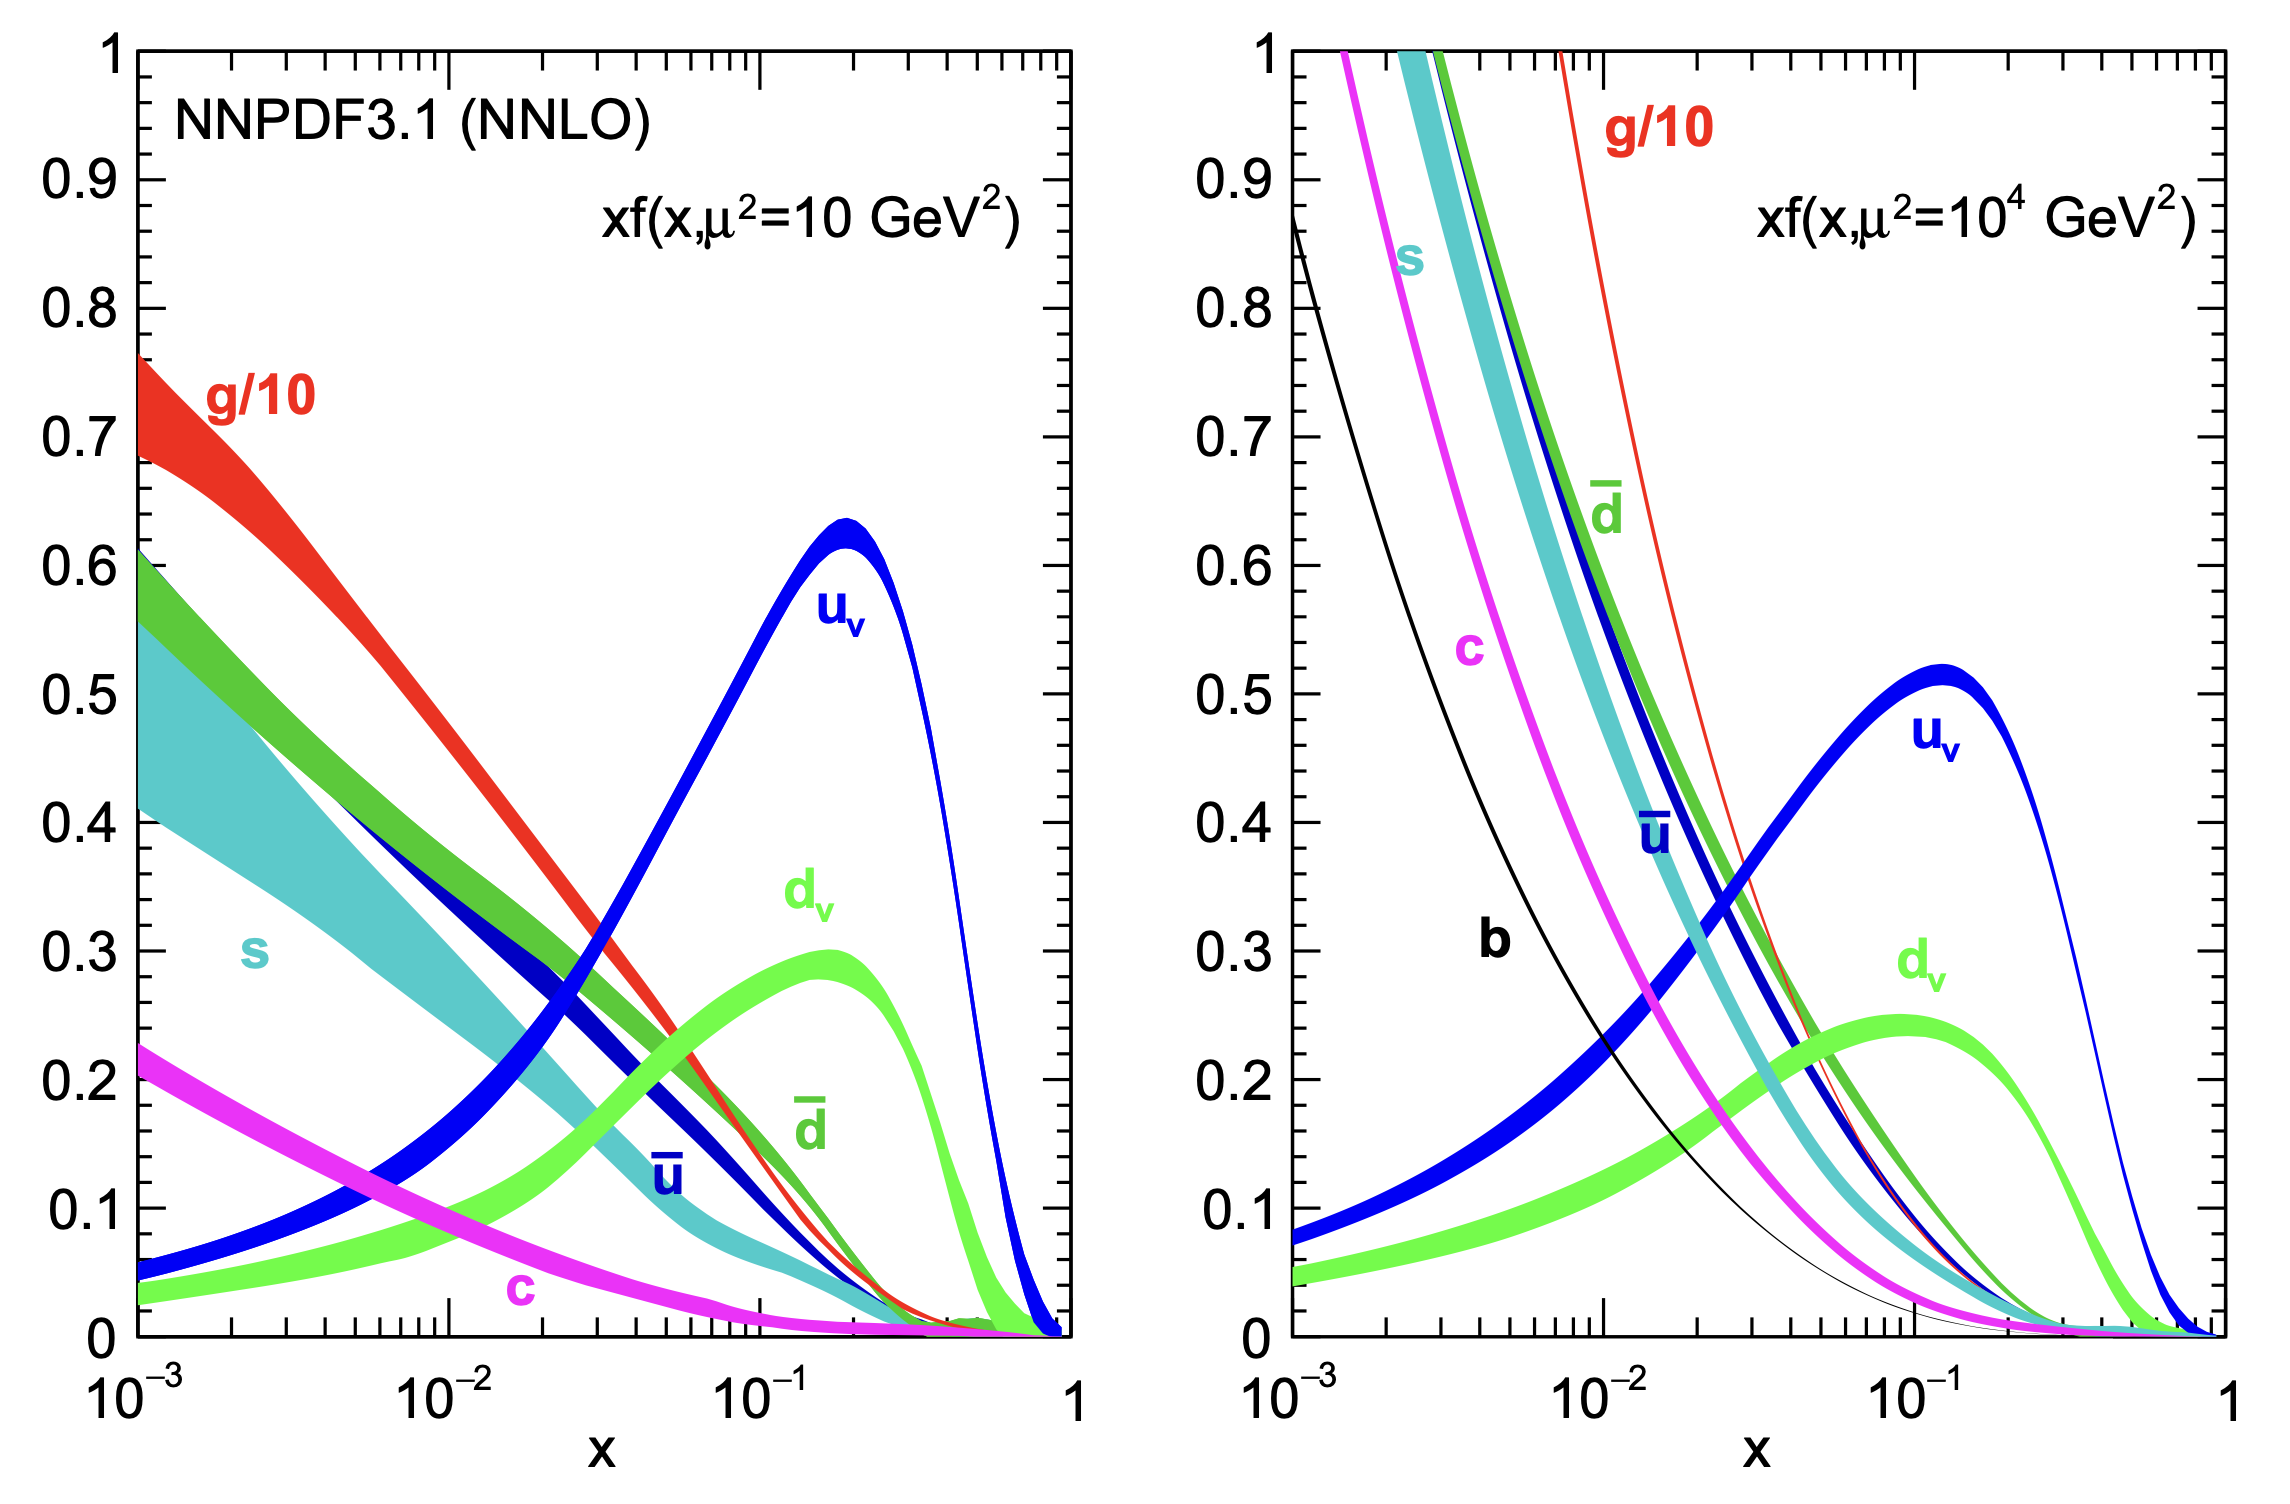
\includegraphics[width=0.8\textwidth]{figures/Part1/QCD/PDF}
 \end{tabular}
 \caption{The NNPDF3.1 \acp{PDF} multiplied by the proton momentum fraction $x$ calculated at at NNLO accuracy in perturbation theory for $\mu^2$ = 10 $\GeV^2$ (left) and $\mu^2$ = 10$^4~\GeV^2$ (right)~\cite{NNPDF:2017mvq}. The gluon \acp{PDF} in both plots are scaled down by a factor of 10 for improved visualization.}
 \label{fig:PDF}
 \end{center}
\end{figure}

Descriptions of the short-distance physics are contained in the third factor of Equation~\ref{eq:master}, $\hat{\sigma}_{ab\rightarrow k}$, which is the partonic cross-section for the production of partonic final states $k$ from initial partons $i$ and $j$. The initial partons $i$ and $j$ can be quarks, anti-quarks, or gluons, and all possible initial states to produce $k$ are summed over and weighted by the probabilities given by the \acp{PDF}. The partonic cross-section is given by:

\begin{equation}
\hat{\sigma}_{ab\rightarrow k}=\frac{1}{2s}\int[\prod_{i=1}^{n}\frac{d^3q_{i}}{(2\pi)^3E_{i}}][(2\pi)^4\delta^4(\sum_{i=1}^{n}q_{i}^{\mu}-(p_{a}+p_{b})^{\mu})]|\mathcal{M}_{ab\rightarrow k}(\mu_{R}^2,\mu_{F}^2)|^2,
\end{equation}

where $\frac{1}{2s}$ is the flux factor with $s$being the squared center of mass energy of the collision. $E_{i}$, $q_{i}$ and $q_{i}^{\mu}$ are the energy, three-, and four-momentum of the parton $i$ in partonic final state $k$, respectively. $p_{a}^{\mu}$ and $p_{b}^{\mu}$ are the four momenta of the initial state partons $a$ and $b$, respectively. $\mathcal{M}_{ab\rightarrow k}(\mu_{R}^2,\mu_{F}^2)$ is the \ac{ME} that characterizes the transition rate of the partonic process $ab\rightarrow k$.

The partonic cross-section is calculated with the perturbative expansions in powers of the strong coupling constant:

\begin{equation}
\label{eq:expand}
\hat{\sigma}_{ab\rightarrow k}=\hat{\sigma}_{0}+\alpha_{s}(\mu_{R}^2)\hat{\sigma}_{1}+\alpha_{s}^{2}(\mu_{R}^2)\hat{\sigma}_{2}+...,
\end{equation}

where the linear and quadratic terms of $\alpha_{s}^{2}(\mu_{R}^2)$ are referred to as the \ac{LO} and \ac{NLO} terms, respectively. 

The last factor in Equation~\ref{eq:master} are the \acp{FF}~\cite{Field:1976ve} that encode information on how partons produced in hard scatterings are turned into colorless bound states $X$, which may be observed in the detector. More specifically, fraction $z$ of the parton momentum is transferred to the hadron $X$, and the associated probability at energy scale $\mu_{F}$ is represented by $D_{k\rightarrow X}(z,\mu_{F}^2)$. Similar to the situation of the \ac{PDF} determination, the fragmentation falls into the nonperturbative regime of \ac{QCD}, which can not be predicted precisely by theoretical methods. Therefore, the \acp{FF} must be extracted from experiments.  

In addition to the cross-section calculations, collider physicists often need simulated events to compare with data. Several main steps are involved in the simulation of the full picture of a hadron collision event before the detector response kicks in. These main steps typically include hard scattering, \ac{PS}, hadronization, underlying event, and unstable particle decay.

Generation of the hard scattering events is usually done by the \ac{ME} event generator, such as \MG~\cite{Alwall:2014hca} and \Pow~\cite{Frixione:2007vw}. Depending on the process in question, these \ac{ME} generators determine the relevant Feynman diagrams and use \ac{MC} methods to generate final-state particles with properties such as particle types, four-momenta, and spins. Each generated event is weighted by the corresponding transition rate, which is calculated numerically using perturbative theory. The \ac{NLO} expansions are commonly used in these perturbative calculations, which typically means one extra parton is involved in the \ac{ME}.

Beyond the \ac{NLO}, higher order \ac{QCD} effects are modeled by the \ac{PS}, which uses splitting functions to characterize the emissions of soft partons by the initial-state and final-state partons. Since the emitted partons can further emit partons themselves, this process will include soft partons with lower and lower energy until perturbative theory breaks down, and finally produces the \acp{PS}. 

The hadronization process takes account of the confinement of partons into the formation of the observed final-state hadrons. The event generators rely on strings or clusters. model for the simulation of this step. 

The underlying event comes from the interactions between those partons in the incoming hadrons that do not directly participate in the hard subprocess. It produces soft hadrons everywhere in the event and contaminates the hard process that was already simulated. 

The last stage of event generation is the sequential decay of those unstable hadrons produced in the hadronization process. One of the commonly used tools to implement \ac{PS} is \PY~\cite{Sjostrand:2014zea}.
\chapter{Beyond the Standard Model}
\label{chap:BSM}

Although the \ac{SM} represents our best understanding of the elementary particles and their interactions, it does contain some deficiencies. On the one hand, it remains silent on some important phenomena, such as gravity, dark matter, and dark energy. On the other hand, several anomalies have emerged from recent experiments, those in the flavor sector in particular. Two of the experimental results in the flavor sector that work against the \ac{SM} and their phenomenological implications are discussed in \autoref{sec:BSM}. \autoref{sec:Leptoquark} introduces the leptoquark model that can be used to explain the unexpected results that occurred in the flavor sector.

\section{BSM Phenomenology}
\label{sec:BSM}

As discussed in \autoref{sec:Flavor}, the renormalizable \ac{SM} Lagrangian exhibits a few continuous global symmetries, namely the $U(1)_{e}\bigotimes U(1)_{\mu}\bigotimes U(1)_{\tau}$ that gives rise to the conservation of lepton family numbers. Unlike gauge symmetries of the \ac{SM}, which arise at the outset of the construction, these global $U(1)$ symmetries emerge accidentally due to the assumption (massless neutrino) that is solely driven by phenomenology. Despite the accidental nature of these symmetries, they have stood up to the tests of almost all particle physics experiments to date.  

In fact, the first and so far the only hint of the broken global symmetries didn't appear until the turn of the century through the oscillation of atmospheric neutrinos \cite{Super-Kamiokande:1998kpq,SNO:2002tuh}. Figure~\ref{fig:SuperK} shows the strong evidence of neutrino oscillations presented by the Super-Kamiokande Collaboration. This remarkable observation directed significant interest from both theorists and experimentalists to the flavor sector of the \ac{SM}. On the one hand, it cements the calls for extensions of the \ac{SM} by demonstrating the mixing of neutrino flavors. On the other hand, it also suggests that the $U(1)$ symmetries are indeed broken, and the \ac{CLFV} is also expected to occur. 

\begin{figure}[tbh!]
 \begin{center}
 \begin{tabular}{c}
 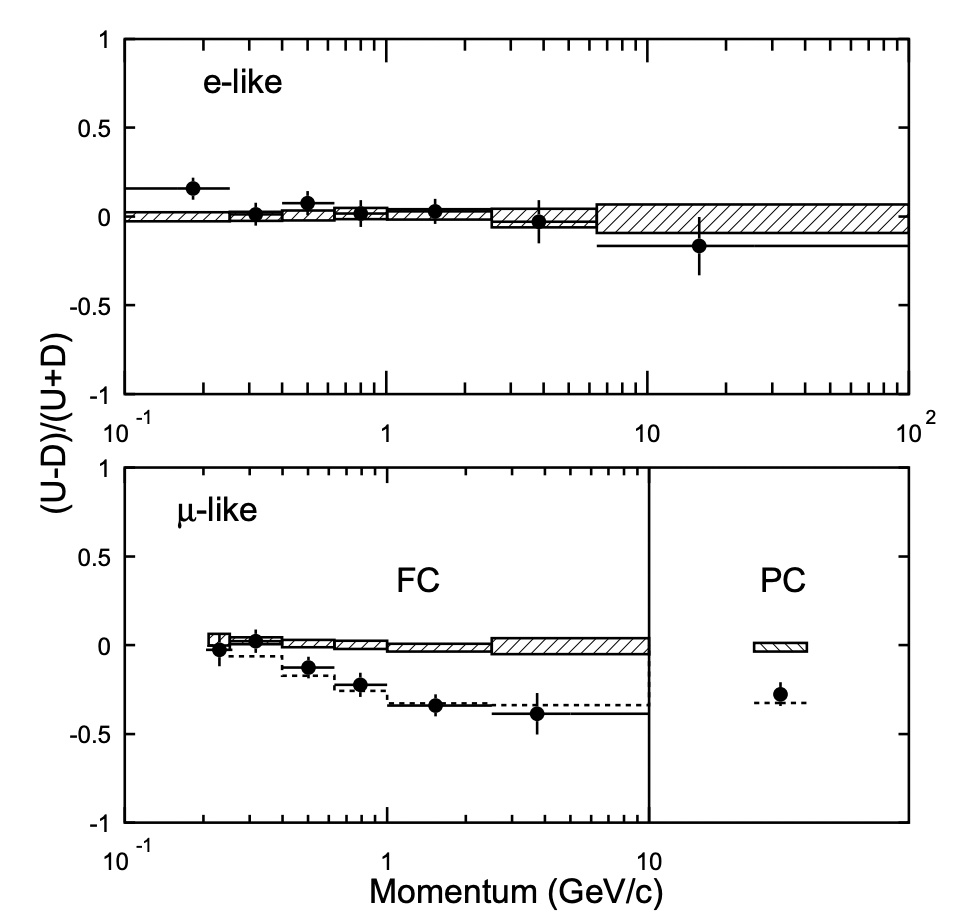
\includegraphics[width=0.6\textwidth]{figures/Part1/BSM/SuperK}
 \end{tabular}
 \caption{Evidence of neutrino oscillation presented by the Super-Kamiokande Collaboration in 1998~\cite{Super-Kamiokande:1998kpq}. The asymmetry in the zenith angle is plotted as a function of momentum for $e$-like events (upper panel) and $\mu$-like events. The data are represented with filled points. The expected distributions under the hypothesis of no neutrino oscillation are shown with filled bands while the dashed line is the expected distribution for the alternative hypothesis.}
 \label{fig:SuperK}
 \end{center}
\end{figure}

Although the exact mechanism behind neutrino mass remains unclear, it can be induced through two distinct ways that only require minimal departures from the original formulation of the \ac{SM}. By adding right-handed neutrino fields, the Yukawa coupling \cite{Weinberg:1967tq} that describes the emergence of Dirac fermion masses can be naturally extended to neutrinos. The neutrino mass can also be realized by introducing an effective operator~\cite{Weinberg:1979sa}, sometimes referred to as the Weinberg operator. This operator gives rise to Majorana neutrino mass terms upon spontaneous symmetry breaking. This operator is however nonrenormalizable, meaning its underlying theory is valid only up to a specific energy scale. Nevertheless, it can be viewed as an effective description of high-energy physics at a low-energy scale. This type of approach is known as the \ac{EFT}, which is discussed further in \autoref{chap:EFT}.

In either case, the mass of neutrinos is accounted for and Equation~\ref{eq:Yukawa} can be subsequently updated to include neutrino mass terms. The presence of massive neutrino fields also means that the \ac{PMNS} matrix introduced in \autoref{sec:Flavor} will no longer be fully diagonal, for the same reason why the \ac{CKM} matrix contains off-diagonal elements. The strength of the neutrino flavor mixing is therefore governed by the off-diagonal elements of the \ac{PMNS} matrix -- a nearly perfect analog to the \ac{CKM} matrix. 

The same \ac{PMNS} matrix can also give rise to the \ac{CLFV} process through loop diagrams involving charged current, as illustrated in Figure~\ref{fig:mutoe}. However, these diagrams are highly suppressed and phenomenologically negligible due to the small neutrino mass relative to the \ac{EW} scale. Therefore, any experimental observation of \ac{CLFV} will be unambiguous evidence of new physics beyond the \ac{SM}.

\begin{figure}[tbh!]
 \begin{center}
 \begin{tabular}{c}
 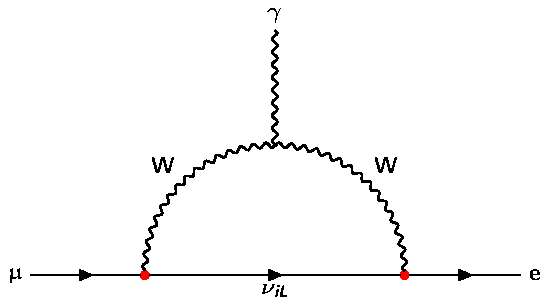
\includegraphics[width=0.7\textwidth]{figures/Part1/BSM/mutoe}
 \end{tabular}
 \caption{Feynman diagram that shows $\upmu\rightarrow$e transition via W loop. The \ac{PMNS} matrix elements enter this diagram through the starting and end points in the W loop, indicated with red dots. The index $i$ runs over lepton generations.}
 \label{fig:mutoe}
 \end{center}
\end{figure}

Recent tests of lepton flavor universality conducted by the \ac{LHCb}~\cite{LHCb:2023zxo} and various other experiments~\cite{HFLAV} in the b$\rightarrow$c transitions established a mild tension (3$\sigma$) with respect to the \ac{SM} predictions. These experiments measured the following ratio of branching fractions:

\begin{equation}
\mathcal{R}(\textsf{D})=\frac{\mathrm{\Gamma}(\textsf{B}\rightarrow\textsf{D}\uptau^{-}\bar{\nu}_{\uptau})}{\mathrm{\Gamma}(\textsf{B}\rightarrow\textsf{D}\upmu^{-}\bar{\nu}_{\upmu})},
\end{equation}

which is sensitive to new physics where the flavor structure is different.

\begin{figure}[tbh!]
 \begin{center}
 \begin{tabular}{c}
 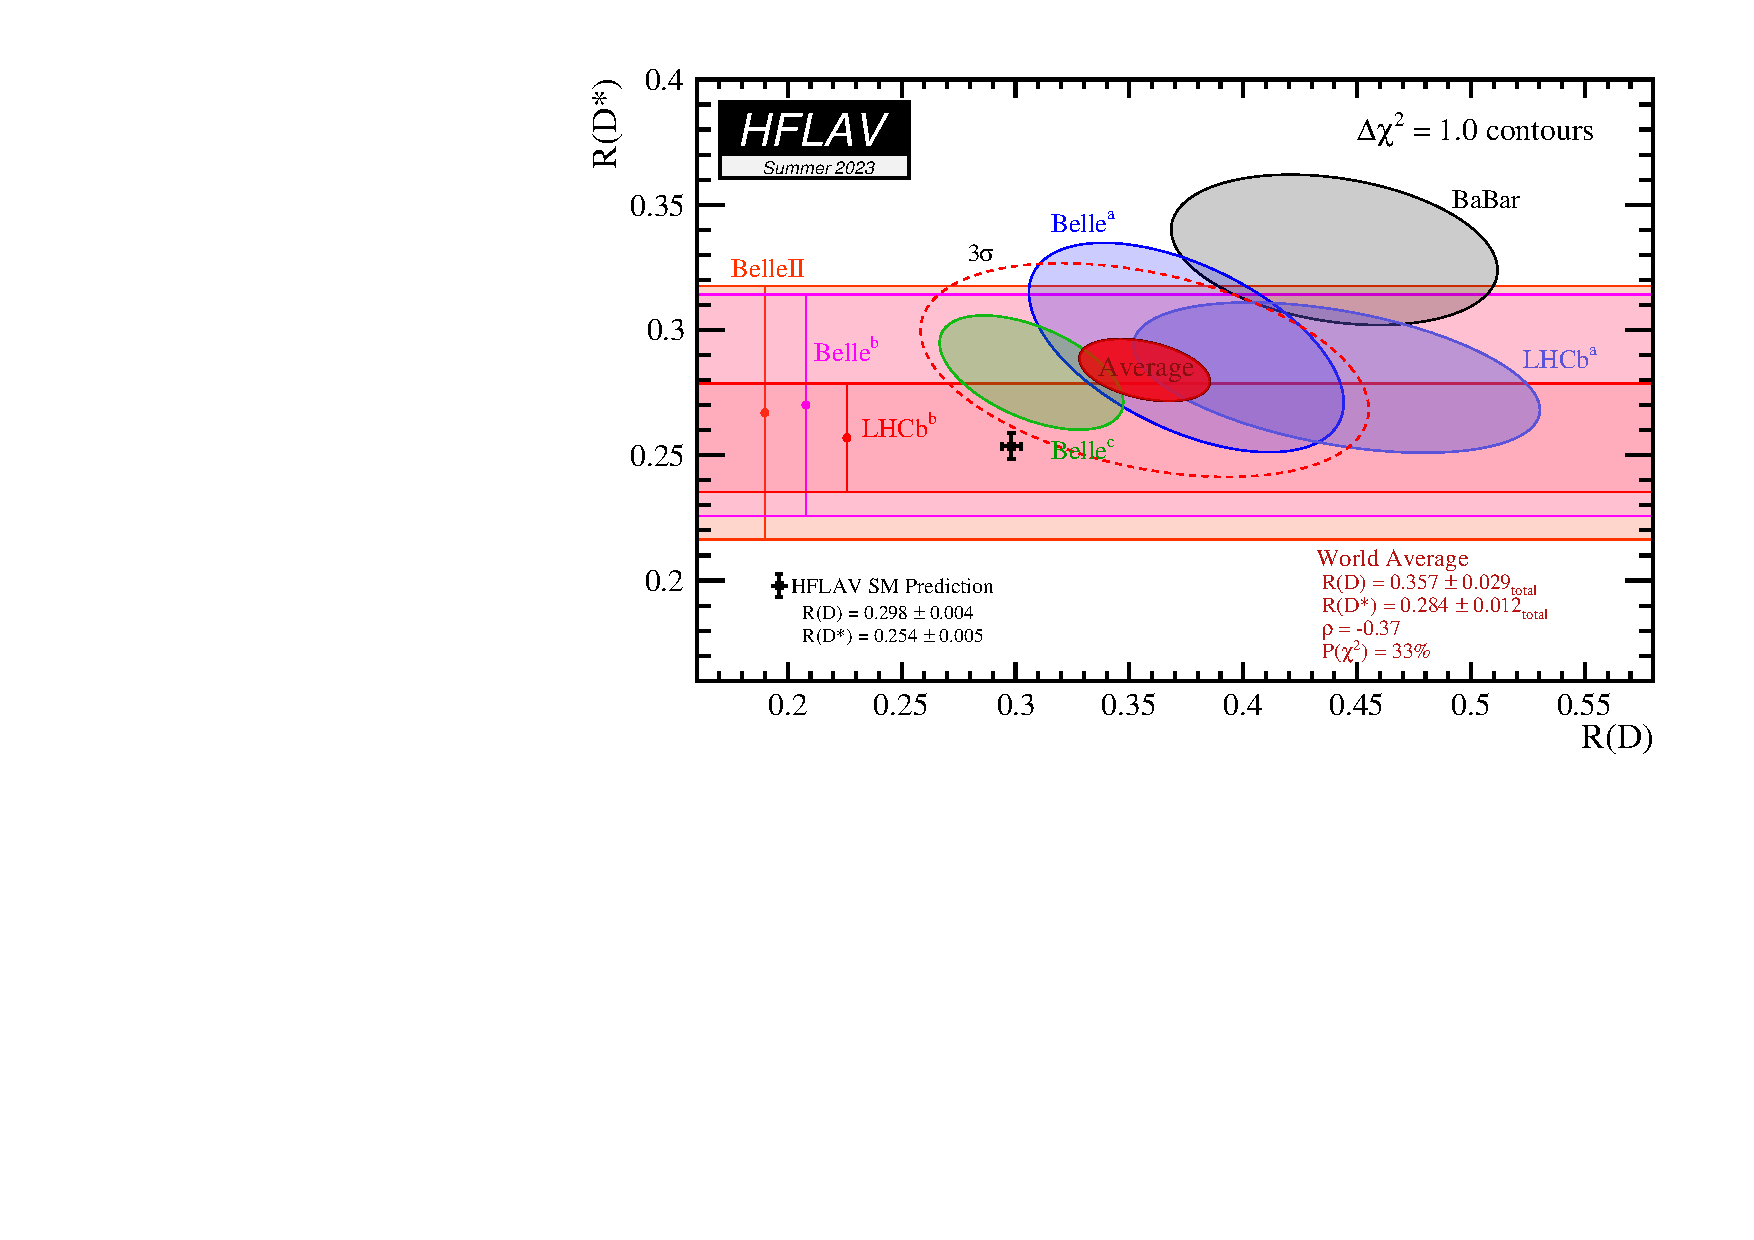
\includegraphics[width=0.7\textwidth]{figures/Part1/BSM/RD}
 \end{tabular}
 \caption{Recent results on $\mathcal{R}(\textsf{D})$ and $\mathcal{R}(\textsf{D}^{*})$ measurements compiled by the HFLAV Group~\cite{HFLAV}. Results are shown in a two-dimensional plane with the x-axis and y-axis representing $\mathcal{R}(\textsf{D})$ and $\mathcal{R}(\textsf{D}^{*})$, respectively. Contours with solid line boundaries represent results published by various experiments. The world average is shown in the middle. The 3$\sigma$ contour is represented with a red dashed line. The \ac{SM} prediction is represented with a data point with error bars.}
 \label{fig:RD}
 \end{center}
\end{figure}

This anomaly is known as the ``$\mathcal{R}(\textsf{D})$'' anomaly and its situation as of Summer 2023 is summarized in Figure~\ref{fig:RD}. As discussed in \autoref{sec:Flavor}, the coupling strength of the weak charged current does not distinguish between lepton flavors. However, results from these measurements seem to suggest the W$\rightarrow\uptau\nu$ decay channel is favored over W$\rightarrow\upmu\nu$ decay channel. Not only did these measurements provide a direct hint towards \ac{LFUV}, it also prompted renewed experimental interest in \ac{CLFV} search since models that accommodate \ac{LFUV} generally give rise to \ac{CLFV} as well~\cite{Glashow:2014iga}. 

\section{Leptoquark Model}
\label{sec:Leptoquark}

Leptoquarks are hypothetical scalar or vector bosons that were first proposed nearly half a century ago~\cite{Pati:1973uk}. They are simultaneously charged with color, isospin, and hypercharge quantum numbers, and thus can mediate lepton-quark couplings. When imposing the \ac{SM} \sm~gauge symmetry, a large pool of possible leptoquark candidates can be reduced to six scalar leptoquarks and six vector leptoquarks~\cite{Dorsner:2016wpm}, which is summarized in Table~\ref{tab:Leptoquark}. 

\begin{table}[th]
\sffamily
\centering
\caption{Possible leptoquark candidates that respect \sm~gauge symmetry, summarized in~\cite{Dorsner:2016wpm}. The spin-0 fields correspond to scalar leptoquark while spin-1 fields correspond to vector leptoquark.}
\begin{tabular}{cccc}
\toprule 
$(SU(3), SU(2), U(1))$ & Spin  & Symbol & Type \\ \midrule
($\bar{\bm{3}}$, $\bm{1}$, -2/3) & 0 & $\bar{S}_{1}$ & $\overline{RR}(\bar{S}_{0}^{\bar{R}})$ \\
($\bar{\bm{3}}$, $\bm{1}$, 1/3) & 0 & $S_{1}$ & $LL(S_{0}^{L})$, $RR(S_{0}^{R})$, $\overline{RR}(S_{0}^{\bar{R}})$ \\
($\bar{\bm{3}}$, $\bm{1}$, 4/3) & 0 & $\tilde{S}_{1}$ & $RR(\tilde{S}_{0}^{R})$ \\
($\bm{\bm{3}}$, $\bm{2}$, 1/6) & 0 & $\tilde{R}_{2}$ & $RL(\tilde{S}_{1/2}^{L})$, $\overline{LR}(\tilde{S}_{1/2}^{\bar{R}})$ \\
($\bar{\bm{3}}$, $\bm{2}$, 7/6) & 0 & $R_{2}$ & $RL(S_{1/2}^{L})$, $LR(S_{1/2}^{R})$ \\
($\bar{\bm{3}}$, $\bm{1}$, -2/3) & 0 & $S_{3}$ & $LL(S_{1}^{L})$\\
\midrule
($\bm{3}$, $\bm{1}$, -1/3) & 1 & $\bar{U}_{1}$ & $\overline{RR}(\bar{V}_{0}^{\bar{R}})$ \\
($\bm{3}$, $\bm{1}$, 2/3) & 1 & $U_{1}$ & $LL(V_{0}^{L})$, $RR(V_{0}^{R})$, $\overline{RR}(V_{0}^{\bar{R}})$ \\
($\bm{3}$, $\bm{1}$, 5/3) & 1 & $\tilde{V}_{1}$ & $RR(\tilde{V}_{0}^{R})$ \\
($\bar{\bm{3}}$, $\bm{2}$, -1/6) & 1 & $\tilde{V}_{2}$ & $RL(\tilde{V}_{1/2}^{L})$, $\overline{LR}(\tilde{V}_{1/2}^{\bar{R}})$ \\
($\bar{\bm{3}}$, $\bm{2}$, 5/6) & 1 & $V_{2}$ & $RL(V_{1/2}^{L})$, $LR(V_{1/2}^{R})$ \\
($\bm{3}$, $\bm{3}$, 1/3) & 1 & $U_{3}$ & $LL(V_{1}^{L})$\\
\bottomrule
\end{tabular}
\vspace{-0.5em}
\label{tab:Leptoquark}
\end{table}

A lot of phenomenological interests have gravitated towards the leptoquark models recently due to the emergence of $\mathcal{R}(\textsf{D})$ anomaly. Taking the $U_{1}$ leptoquarks as an example. Assuming they only interact with left-handed fermions, the interaction term can be written as:

\begin{equation}
\lambda\beta^{ij}_{L}\bar{Q}_{L}^{i}\gamma^{\mu}L_{L}^{j}U_{1\mu},
\end{equation}

where $\lambda$ is the coupling strength, and $\beta^{ij}_{L}$ is a 3$\times$3 matrix that encodes the flavor structure of $U_{1}$ interactions. This term can contribute at the tree level to the b$\rightarrow$c transitions where the anomaly is reported. A side-by-side comparison of Feynman diagrams for the \ac{SM} and leptoquark contributions to this process is shown in Figure~\ref{fig:Leptoquark}.

\begin{figure}[tbh!]
 \begin{center}
 \begin{tabular}{cc}
 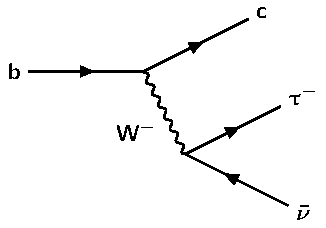
\includegraphics[width=0.45\textwidth]{figures/Part1/BSM/SMbtoc}&
 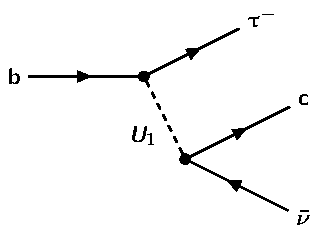
\includegraphics[width=0.45\textwidth]{figures/Part1/BSM/U1}\\
 \end{tabular}
 \caption{Representative Feynman diagram for tree-level $\textsf{b}\rightarrow\textsf{c}\uptau\nu$ transition. The \ac{SM} contribution is shown on the left. Possible contributions from the $U_{1}$ leptoquark, represented with a dashed line in the diagram, are shown on the right.}
 \label{fig:Leptoquark}
 \end{center}
\end{figure}

An explanation of the $\mathcal{R}(\textsf{D})$ anomaly is possible if $U_{1}$ leptoquarks interact strongly with the third generations while leaving out or interacting very weakly with the first and second generations. In other words, a $\beta^{ij}_{L}$ matrix of the form

\begin{equation}
\begin{pmatrix}
0 & 0 & 0\\
0 & \mathcal{O}(0.01) & \mathcal{O}(0.1)\\
0 & -\mathcal{O}(0.1) & 1\\
\end{pmatrix},
\end{equation}

could be used to explain the $\mathcal{R}(\textsf{D})$ anomaly, as pointed out by Ref.~\cite{Cornella:2021sby}.

Secondly, the leptoquark model provides an interesting connection between the $\mathcal{R}(\textsf{D})$ anomaly and flavor-changing phenomena at a higher energy scale. For example, $\mathcal{R}(\textsf{D})$ anomaly can also be explained by the $S_1$ leptoquark listed in Table~\ref{tab:Leptoquark}. Because $S_1$ can interact with left-handed fields, the b quark and neutrino in the interaction vertex can be replaced with a top quark and a muon, as illustrated in Figure~\ref{fig:S1}. This results in the flavor-violating t$\rightarrow\ell\ell^{\prime}$q decay, which is strongly suppressed in the \ac{SM} by the mass hierarchy of both quarks and leptons. It was suggested in Ref.~\cite{Kim:2018oih} that the $\mathcal{R}(\textsf{D})$ anomaly, if true, can give rise to a sizable rate of \ac{CLFV} events, which reaches $\mathcal{O}(10^{-6})$ at tree-level for t$\rightarrow\ell\ell^{\prime}$c process involving a top quark.

\begin{figure}[tbh!]
 \begin{center}
 \begin{tabular}{cc}
 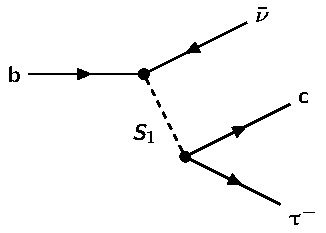
\includegraphics[width=0.45\textwidth]{figures/Part1/BSM/S1}&
 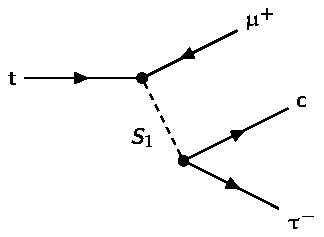
\includegraphics[width=0.45\textwidth]{figures/Part1/BSM/S1x}\\
 \end{tabular}
 \caption{Feynman diagrams of processes mediated by $S_1$ leptoquark, represented with a dashed line in both diagrams. The left diagram shows a possible explanation for $\mathcal{R}(\textsf{D})$ anomaly offered by the $S_1$. The same $S_1$ can give rise to \ac{CLFV} in the top quark sector, which is shown on the right.}
 \label{fig:S1}
 \end{center}
\end{figure}

Finally, the \ac{CERN} \ac{LHC} can provide sensitivity to \ac{CLFV} searches in two- or three-body decays of heavy particles, X$\rightarrow\ell\ell^{\prime}$(Y), and in heavy-particle production, pp$\rightarrow\ell\ell^{\prime}$X. Here, X refers to a heavy \ac{SM} particle such as a top quark or a Higgs, W, or Z boson, Y denotes an additional generic \ac{SM} particle. For \ac{CLFV} processes involving the heaviest of all elementary particles, the top quark, competitive sensitivity is predicted at the \ac{LHC} compared to previous bounds on such interactions~\cite{Davidson:2015zza}. Therefore, a search for \ac{CLFV} in the top quark sector at the \ac{LHC} could shed light on these flavor anomalies and further our understanding of the broken global symmetries.
\chapter{Effective Field Theory}
\label{chap:EFT}

The concept of effective interactions has been around for nearly a century since Fermi first introduced it in 1933~\cite{Fermi:1933jpa} to explain the $\upbeta$ decay. The modern approach to effective interactions builds on the assumption that there is a separation between energy scales of different physics phenomena. When describing low-energy physics, the heavy mediators can be approximated to be point-like, and thus described by an effective coupling. This type of approach, collectively known as \ac{EFT}, has been very successful in simplifying calculations and describing low-energy experiments with stunning precisions. Depending on the energy scale at which \acp{EFT} are operating, they can be classified into different versions. One version of the \ac{EFT} that operates below the \ac{EW} scale and integrates out all the heavy fields is called the \ac{LEFT}, which is described in \autoref{sec:LEFT}. Another version of the \ac{EFT} that operators above the \ac{EW} scale is called the \ac{SMEFT}. It retains all the \ac{SM} fields and \sm~gauge symmetry. A description of the \ac{SMEFT} is given in \autoref{sec:SMEFT}.

\section{Low-Energy EFT}
\label{sec:LEFT}

It is safe to say that Fermi did not have a complete description of the weak interactions in 1933. Instead, he constructed a phenological model to explain the $\upbeta$ decay. In his theory, he modified the \ac{QED} to include the following interaction vertex between four fermion fields:

\begin{equation}
-\frac{G_{\textsf{F}}}{\sqrt{2}}(\bar{\psi}_{\textsf{p}}\mathrm{\Gamma}\psi_{\textsf{n}})(\bar{\psi}_{\textsf{e}}\mathrm{\Gamma}\psi_{\nu})
\end{equation}

where $G_{\textsf{F}}$ is known as the Fermi constant, $\psi$ are Dirac fields that represent up quark (proton), down quark (neutron), electron, and electron neutrino. $\mathrm{\Gamma}$ is a 4$\times$4 matrix that encodes the Lorentz structure of the effective interaction. 

From the point of view of the \ac{SM}, the $\upbeta$ decay is described by the charged-current interaction, whose amplitude in perturbative theory can be derived from the Lagrangian specified in Equation~\ref{eq:LCC}:

\begin{equation}
\label{eq:beta}
\frac{1}{8}(\bar{u}\mathrm{\Gamma}d)\frac{g^2}{q^2-m_{W}^2}(\bar{e}\mathrm{\Gamma}\nu),
\end{equation}

where $q$ and $m_W$ are the momentum and mass of the W propagator, respectively, and $g$ is the strength of the $SU(2)_{L}$ gauge interaction as mentioned in \autoref{sec:Gauge}.

Because $m_W\approx$ 80.4 GeV, which is considered to be a lot higher than the energy scale associated with the $\upbeta$ decay, the momentum of the W boson can be ignored and Equation~\ref{eq:beta} reduces to:

\begin{equation}
\label{eq:beta2}
-\frac{g^2}{8m_{W}^2}(\bar{u}\mathrm{\Gamma}d)(\bar{e}\mathrm{\Gamma}\nu),
\end{equation}

which is exactly the Fermi's theory with:

\begin{equation}
\frac{G_{\textsf{F}}}{\sqrt{2}}=\frac{g^2}{8m_{W}^2}.
\end{equation}

As illustrated in Figure~\ref{fig:FermiEFT}, Fermi's theory of weak interaction works very well at low energy. However, it ultimately breaks down when the momentum transfer is high enough. 

\begin{figure}[tbh!]
 \begin{center}
 \begin{tabular}{cc}
 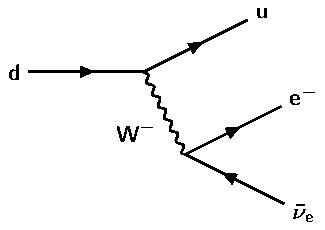
\includegraphics[width=0.45\textwidth]{figures/Part1/EFT/BetaDecay}&
 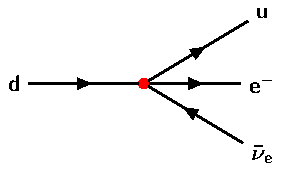
\includegraphics[width=0.45\textwidth]{figures/Part1/EFT/FermiTheory}\\
 \end{tabular}
 \caption{Representative Feynman diagrams for $\upbeta$ decay. The \ac{SM} description of this phenomenon with a massive weak mediator is illustrated on the left. At low energy, the heavy weak boson is approximated to be point-like in Fermi's theory of weak interactions, which is illustrated on the right. The effective coupling between four fermions indicated with a red dot, can be used to describe the same phenomenon.}
 \label{fig:FermiEFT}
 \end{center}
\end{figure}

The \ac{LEFT} that we know today is not that different from Fermi's original theory of weak interactions. It operates below the \ac{EW} scale, where the gauge symmetry of the \ac{SM} reduces to $SU(3)_{C}\bigotimes U(1)_{EM}$. It makes no explicit assumptions about the structure of the theory at higher energy. Except for the gauge bosons, the Higgs boson, and the top quark, all other fields are considered in the \ac{LEFT}. 

The \ac{LEFT} is usually deployed in a ``bottom-up'' way to model high-energy physics, whose structure is not yet known. For example, assuming new physics at a very high energy scale is responsible for the $\mathcal{R}(\textsf{D})$ anomaly described in \autoref{sec:BSM}, the phenomenon observed at low-energy experiments can be therefore parameterized by the \ac{LEFT}, as illustrated in Figure~\ref{fig:LEFT}.

\begin{figure}[tbh!]
 \begin{center}
 \begin{tabular}{cc}
 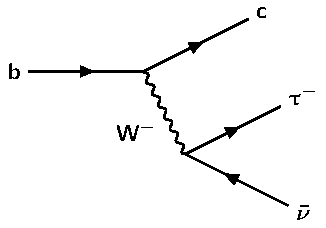
\includegraphics[width=0.45\textwidth]{figures/Part1/BSM/SMbtoc}&
 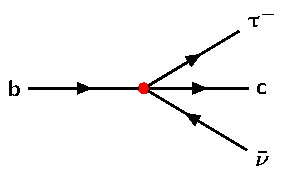
\includegraphics[width=0.5\textwidth]{figures/Part1/EFT/LEFT}
 \end{tabular}
 \caption{Representative Feynman diagram for b$\rightarrow$c transtion in the \ac{SM} (left). This process might also be enhanced by new physics with a much higher energy scale. The potential contributions from new physics can therefore be described by an effective coupling between four fermions, which is illustrated on the right.}
 \label{fig:LEFT}
 \end{center}
\end{figure}

\section{Standard Model EFT}
\label{sec:SMEFT}

The \ac{SM} can also be viewed as an \ac{EFT} as it is commonly accepted that it is not valid up to an arbitrarily high energy scale. This view leads to a different version of \ac{EFT}, known as the \ac{SMEFT}. The \ac{SMEFT} builds higher dimensional operators out of \ac{SM} fields to systematically study \ac{SM} deviations. These higher dimensional operators respect \sm~gauge symmetry and are added to \ac{SM} Lagrangian:

\begin{equation}
\label{eq:SMEFT}
\mathcal{L}_{\textsf{SMEFT}}=\mathcal{L}_{\textsf{SM}}^{(4)} + \frac{1}{\Lam}\WC{(5)}{}\OP{(5)}{}+ \frac{1}{\Lam^2}\sum_{a}\WC{(6)}{a}\OP{(6)}{a} + ...,
\end{equation}  

where $\mathcal{L}_{\text{SM}}^{(4)}$ is the renormalizable Lagrangian of the \ac{SM}. The $\OP{(n)}{}$ denote dimension-n nonrenormalizable operators, and $\WC{(n)}{}$ are the corresponding Wilson coefficients. The high dimensional operators are suppressed by powers of a mass scale $\Lambda$ where new physics is presumed to emerge. 

The only \ac{SM} gauge-invariant operator at dimension-five is the Weinberg operator~\cite{Weinberg:1979sa}, illustrated in Figure~\ref{fig:Dim5}, of the following form

\begin{equation}
\OP{(5)}{}=(\phi\cdot\bar{L})(L\cdot\phi),
\end{equation}

where $\phi$ is the Higgs doublet mentioned in \autoref{sec:Higgs}. 

\begin{figure}[tbh!]
 \begin{center}
 \begin{tabular}{c}
 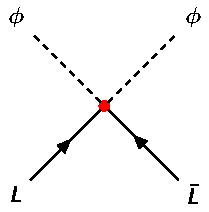
\includegraphics[width=0.45\textwidth]{figures/Part1/EFT/Dim5}
 \end{tabular}
 \caption{Illustration of the lepton-number violating Weinberg operator.}
 \label{fig:Dim5}
 \end{center}
\end{figure}

This operator gives rise to the Majorana mass terms for neutrinos upon \ac{EW} symmetry breaking:

\begin{equation}
m_{\textsf{Majorana}}=\WC{(5)}{}\frac{v^2}{\Lam},
\end{equation}

where $v$ is the vacuum expectation value mentioned in \autoref{sec:Higgs}.

Many more dimension-six operators are invariant under the \ac{SM} gauge transformations. They can be classified by the so-called Warsaw basis~\cite{Grzadkowski:2010es}. These operators are more relevant to this thesis as they can be formed by four fermionic fields that facilitate the flavor-violating $\ell\ell^{\prime}$qt interactions. A summary of these four-fermion operators is given in \autoref{sec:Signals}.

